\documentclass[11pt]{article}

\usepackage[margin=1in]{geometry}
\usepackage{amsmath}
\usepackage{amssymb}
\usepackage{graphicx}
\usepackage{booktabs}
\usepackage{hyperref}
\usepackage{url}

\title{Comparative Analysis of Conserved and Non-Conserved Ising Kinetics: \\
Microstructural Evolution, Anisotropic Coarsening, and Interfacial Dissipation}
\author{Django Thompson}
\date{\today}

\begin{document}
\maketitle

\noindent\textit{Working draft, 14 September 2026. This manuscript has not
been peer reviewed or independently checked in full by the student. Code,
analysis, figures and draft prose received substantial generative-AI
assistance; the contribution record is in the repository. The tracked PDF is
older than this source.}

\begin{abstract}
Microstructures evolve differently depending on whether the quantity that
defines them is free to change locally or is fixed globally. I built two
Monte Carlo engines for the two-dimensional Ising model to study this
directly: one with Metropolis single-spin-flip dynamics, in which the
order parameter is not conserved, and one with spin-exchange (Kawasaki)
dynamics, in which it is conserved exactly. After quenching each below its
respective critical temperature, I extract the
characteristic domain size $L(t)$ from the equal-time spatial spin correlation function and
fit its growth. The non-conserved case gives a finite-window exponent close to the
curvature-driven Lifshitz--Allen--Cahn prediction $L(t)\propto t^{1/2}$; the
conserved case grows more slowly in the tested window; these runs do not
establish the diffusion-limited Lifshitz--Slyozov asymptote
$L(t)\propto t^{1/3}$. I then generalise the
conserved model to unequal couplings $J_x \neq J_y$, a simple stand-in for
direction-dependent interfacial energy, and show it produces markedly
elongated domains. This gives a controlled way to explore directional
interface costs, not a prediction of a textured alloy. I then test a more
subtle late-stage prediction: that the conserved
model's asymptotic growth exponent is independent of composition within
the scaling regime, even when moving from a symmetric, bicontinuous quench to a dilute, off-critical quench in
which the minority phase forms isolated droplets, even though the
morphology changes completely. A sweep over six initial concentrations
finds an approximately flat *finite-window* effective-exponent plateau down
to $c=0.10$, with additional slowing at the most dilute point, $c=0.06$;
this is not a test of the asymptotic limit. A periodic
connected-component analysis of the simulated droplet-size distribution in
the dilute regime is compared against the closed-form
Lifshitz--Slyozov--Wagner prediction. Finally, by
tracking the heat exchanged with the thermal bath at every accepted move,
I compute the bath entropy-flow rate $\dot S_{\mathrm{bath}}(t)$ for both
models and show it falls by several orders of magnitude as each system
coarsens. This heat-based quantity is a dissipation proxy, not the total
stochastic entropy production, which also requires the system-entropy change.
\end{abstract}

\section{Introduction}

Most useful materials are not single crystals sitting quietly in
equilibrium. Steels, magnetic thin films, and polymer blends are all
microstructures caught partway through relaxing towards some more ordered
state, and it is usually that half-relaxed microstructure -- the size,
shape, and spacing of the grains or precipitates in it -- that determines
whether the material is strong, brittle, or magnetically useful. Working
out how that microstructure changes with time after a material is
processed (cast, quenched, annealed) is the basic problem of
\emph{phase-ordering kinetics}, and it turns out that a huge amount can be
learned from a model far simpler than any real alloy: the Ising model.

The Ising model is normally introduced as a toy magnet, and that is a
perfectly good way to think about it. But it is also, without much
translation needed, a lattice model of a binary mixture: a `$+1$' spin is
an A atom, a `$-1$' spin is a B atom, and the coupling between neighbouring
spins gives a lattice-gas representation of an idealised binary mixture.
The same pair-energy expression can be read in either language, but a real
alloy also has diffusion mechanisms, crystal structure, elastic effects and
interactions missing here. Changing the allowed move creates two different
kinetic models:

\begin{itemize}
\item If a ``move'' is flipping a single spin, nothing stops the total
magnetisation from drifting. Physically, this is what happens when a
non-conserved quantity orders itself out of a disordered state --
magnetic domains forming as a thin film cools below its Curie point. The
curvature-driven growth mechanism is also relevant to grain growth, although
two Ising states do not describe the many grain orientations in a real
polycrystal. This
is usually called \textbf{Model A} dynamics, in the naming scheme
Hohenberg and Halperin set out for dynamic critical phenomena
\cite{HohenbergHalperin1977}.
\item If a ``move'' is instead exchanging two neighbouring spins, the total
magnetisation cannot change at all -- it is conserved by construction.
This is a minimal conserved model for \textbf{phase separation in a binary
mixture}: the numbers of A and B sites cannot change, so an A-rich region
can only grow by material moving from elsewhere. This is \textbf{Model B}
dynamics in the same scheme. Nearest-neighbour swaps do not reproduce an
alloy's atomistic diffusion route, but they allow the conservation-limited
coarsening mechanism to be studied.
\end{itemize}

The motivating theory is that conserving the order parameter can change
the late-stage coarsening law. The historical Model A and anisotropic Model B
baselines below use different sizes, couplings and quench conditions, so
their numerical slopes alone are not a controlled measurement of the
effect of conservation. I built both simulations from scratch in
Python (accelerated with Numba, since a naive Python Monte Carlo loop is
far too slow to reach interesting length and time scales), extended the
conserved model to allow direction-dependent coupling as a simple model of
crystallographic anisotropy, and built two interactive dashboards (a
desktop one and a browser one) so the coarsening process can be watched as
it happens rather than only inspected after the fact in a saved CSV file.
Everything reported below, including every number quoted, comes from
runs of that code, and the code itself is openly available
\cite{CodeRepo}.

\section{Theoretical and Computational Foundations}

\subsection{The anisotropic Ising Hamiltonian}

Each site $i$ of an $L\times L$ square lattice carries a spin
$\sigma_i \in \{-1,+1\}$, with periodic boundary conditions so that the
lattice has no edges. For most of this project the coupling between
neighbours is the same in both lattice directions, but for the anisotropy
study in Section~4 I let it differ:
\begin{equation}
H = -J_x \sum_{\langle i,j\rangle_x} \sigma_i \sigma_j \;-\; J_y \sum_{\langle i,j\rangle_y} \sigma_i \sigma_j,
\label{eq:hamiltonian}
\end{equation}
where $\langle i,j\rangle_x$ and $\langle i,j\rangle_y$ are sums over
horizontal and vertical nearest-neighbour bonds respectively, each counted
once. Setting $J_x = J_y = J$ recovers the ordinary isotropic Ising model.
Physically, $J_x \neq J_y$ is a simple stand-in for direction-dependent
interfacial energy. It creates a directional bond cost, not a model of
crystallographic elasticity or processing texture.

\subsection{Equilibrium thermodynamics}

At a fixed temperature $T$, the system explores configurations according
to the Boltzmann distribution,
\begin{equation}
P(\sigma) = \frac{e^{-\beta H(\sigma)}}{Z}, \qquad \beta = \frac{1}{k_B T}, \qquad Z = \sum_\sigma e^{-\beta H(\sigma)},
\label{eq:boltzmann}
\end{equation}
where $Z$ is the partition function (the normalising sum over every
possible spin configuration). Equilibrium is the state that minimises the
Helmholtz free energy $F = E - TS$, not the energy alone -- entropy
matters, and it matters more as $T$ increases. At low temperature the
energy term wins and an unconstrained system prefers an ordered, all-aligned
state (while the conserved mixture must retain its fixed composition); at
high temperature the entropy term wins and disorder is preferred, because
there are astronomically more disordered configurations than ordered
ones. In between, there is a temperature at which the two effects balance
so finely that the transition between them is sharp rather than gradual.
For the isotropic square-lattice Ising model this critical temperature is
known exactly, from Onsager's 1944 solution \cite{Onsager1944}:
\begin{equation}
T_c = \frac{2J}{\ln(1+\sqrt2)} \approx 2.269\ J/k_B.
\label{eq:tc}
\end{equation}
For the anisotropic case, $T_c$ is instead the root of
\begin{equation}
\sinh\!\left(\frac{2J_x}{k_B T_c}\right)\sinh\!\left(\frac{2J_y}{k_B T_c}\right) = 1,
\label{eq:tc-aniso}
\end{equation}
which I solve numerically and which reduces to Eq.~\eqref{eq:tc} when
$J_x=J_y$. I use this both to sanity-check the simulation against an exact
result and to set consistent quench temperatures for the anisotropic runs.

\subsection{Regular-solution spinodal implied by the lattice coupling}

The conserved model also has a direct binary-alloy reading, in which a
$+1$ spin is an A atom, a $-1$ spin is a B atom, and
$c=(1+m)/2$ is the A-atom concentration. This makes it possible to connect
the kinetic simulations to a simple phase-diagram construction rather than
only to a magnetic critical temperature. In a bond of direction $d\in\{x,y\}$,
the Ising energy is $-J_d$ for either like pair (A--A or B--B) and $+J_d$
for an unlike A--B pair. Thus an unlike bond costs $2J_d$ relative to a
like bond. Counting one horizontal and one vertical bond per lattice site,
then adding ideal configurational entropy, gives the Bragg--Williams
regular-solution free energy per site
\begin{equation}
f(c,T) = k_B T\left[c\ln c+(1-c)\ln(1-c)\right]+\Omega c(1-c),
\qquad \Omega=4(J_x+J_y).
\label{eq:regular-solution-free-energy}
\end{equation}
The spinodal is the locus at which this homogeneous free energy loses local
stability, $\partial^2 f/\partial c^2=0$:
\begin{equation}
k_B T_s(c)=2\Omega c(1-c)=8(J_x+J_y)c(1-c).
\label{eq:regular-solution-spinodal}
\end{equation}
For the isotropic concentration study ($J_x=J_y=1$), Eq.~\eqref{eq:regular-solution-spinodal}
becomes $T_s=16c(1-c)$ and has a mean-field maximum $T_c^{\rm RS}=4J/k_B$ at
$c=0.5$; for the anisotropic baseline ($J_x=1$, $J_y=0.5$), it is
$T_s=12c(1-c)$ with maximum $3J/k_B$. The plotting script evaluates these
identities numerically before rendering Fig.~\ref{fig:spinodal}.

Figure~\ref{fig:spinodal} places the actual Model B temperature paths on
this mean-field diagram. The composition sweep begins above the spinodal at
$T_i=6.808$ and finishes at $T_f=1.475$. Its $c\ge0.15$ end points lie
inside the mean-field spinodal, whereas $c=0.10$ and $0.06$ lie outside
it on the metastable side of this approximation. Droplet morphology alone
does not identify a nucleation mechanism: $c=0.15$ is droplet-rich but
remains inside this mean-field spinodal. The curve is not the exact
two-dimensional Ising binodal:
its $T_c^{\rm RS}=4J/k_B$ deliberately differs from Onsager's exact
$T_c=2.269J/k_B$. Model A is not placed on this alloy diagram because its
Metropolis single-spin-flip moves do not conserve composition.

\begin{figure}[t]
\centering
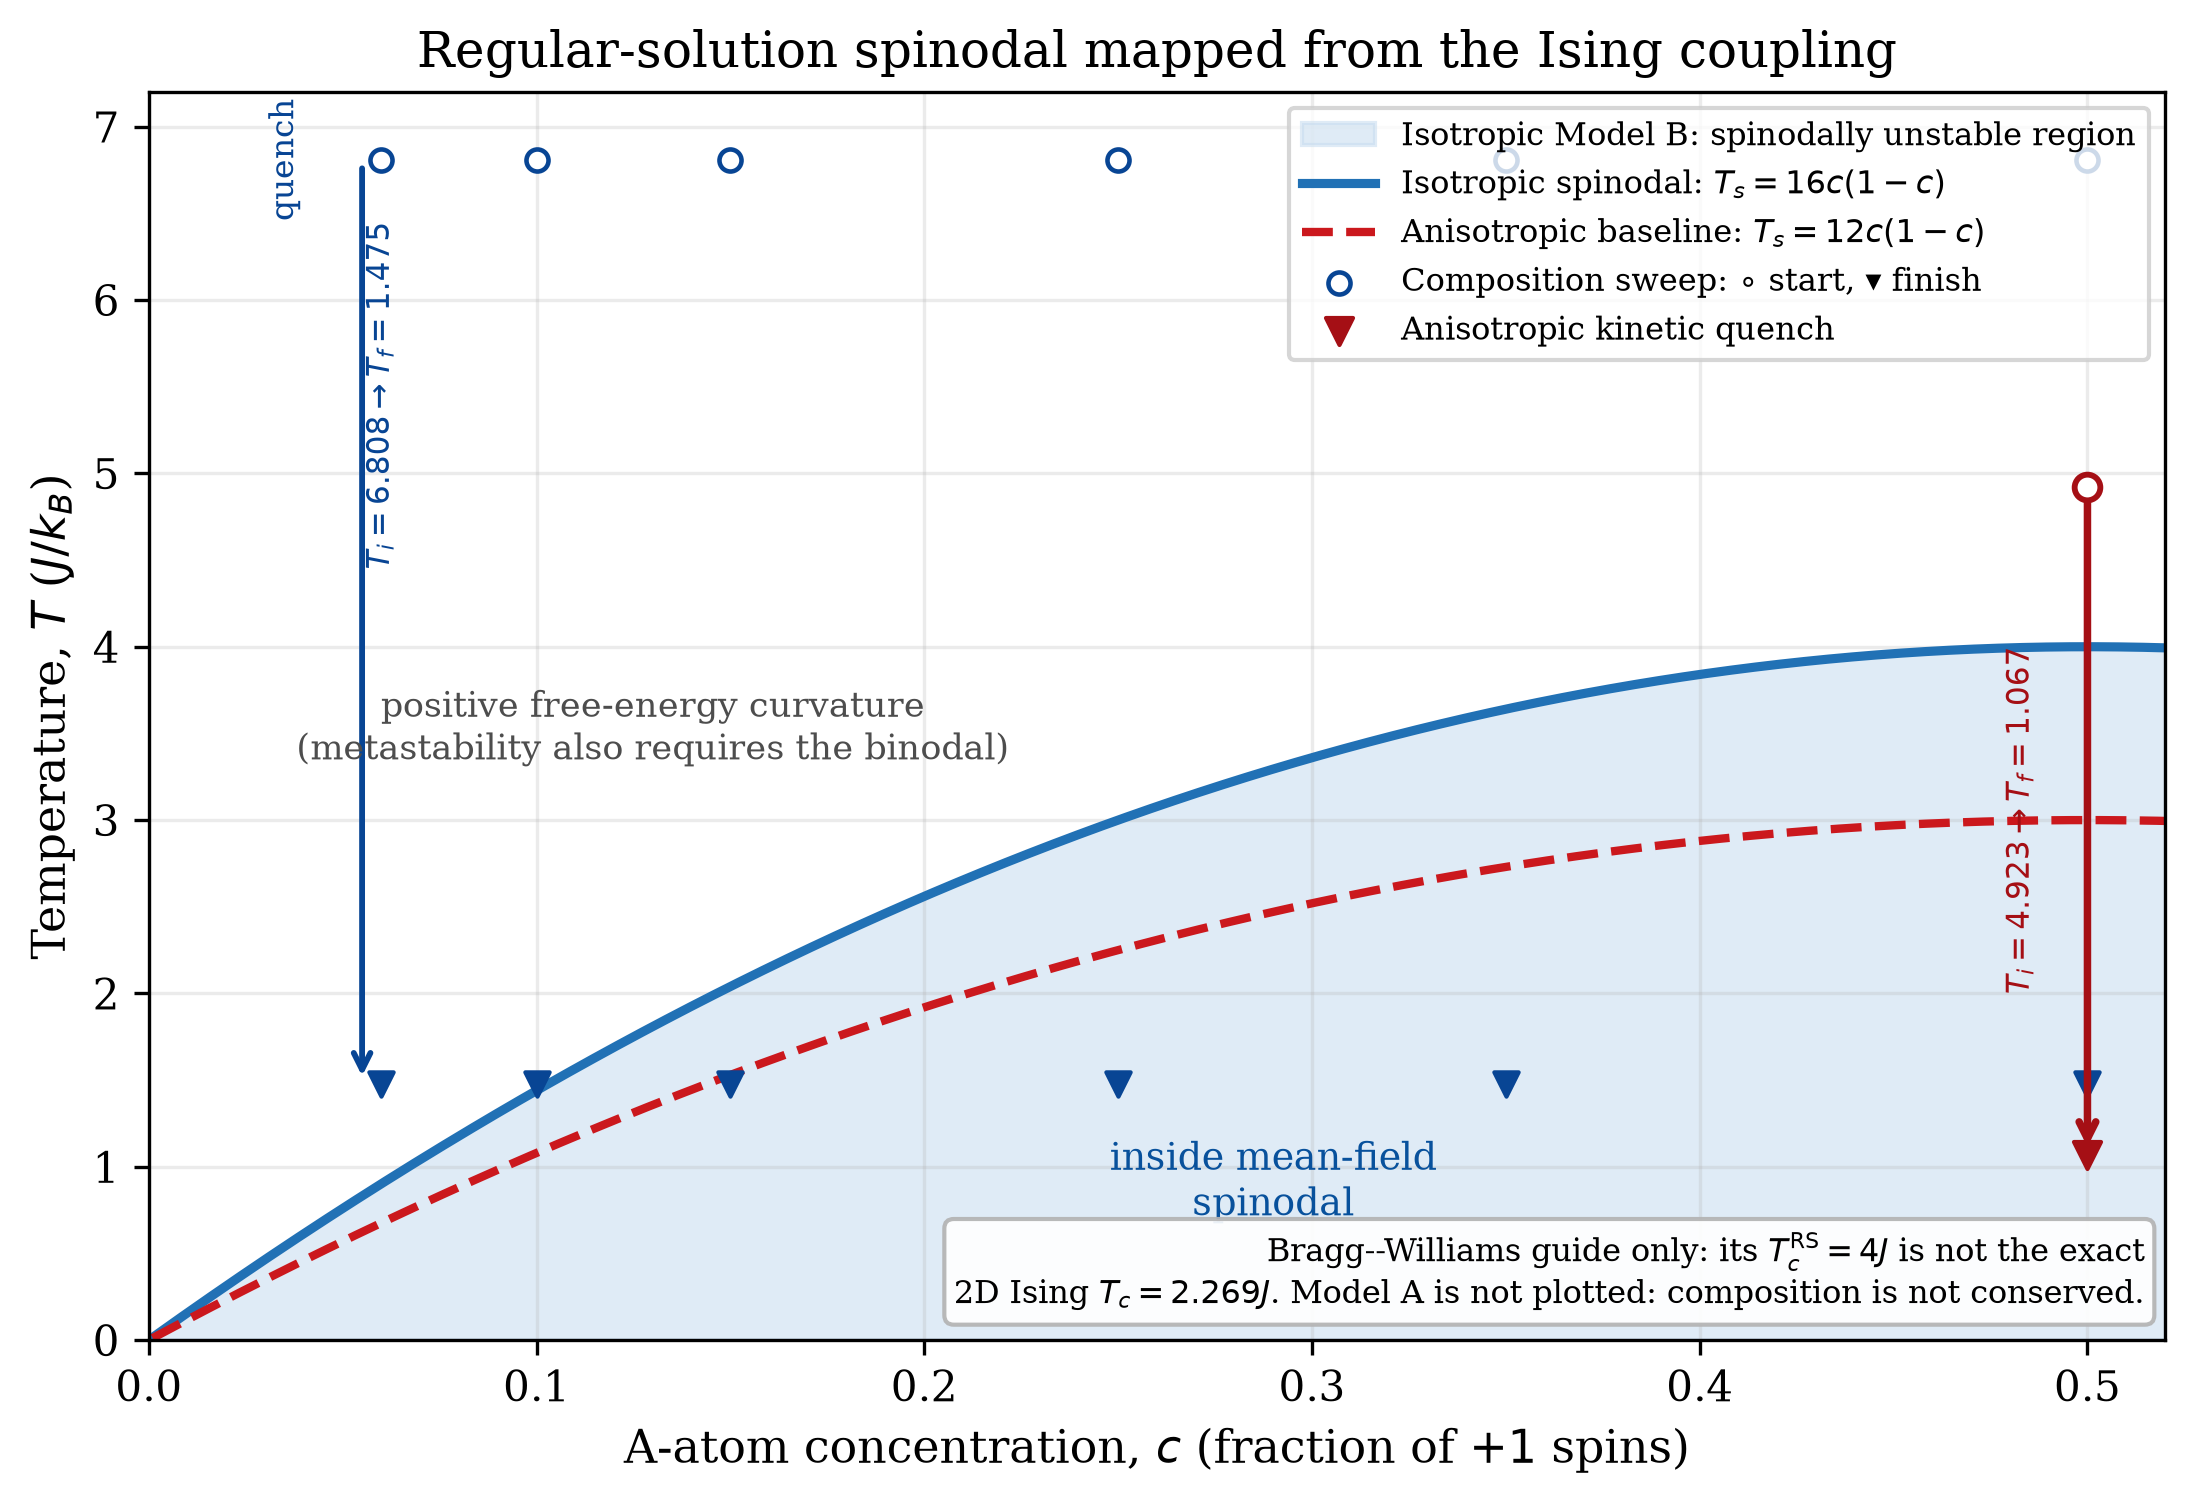
\includegraphics[width=\textwidth]{../figures/fig_regular_solution_spinodal.png}
\caption{Bragg--Williams regular-solution spinodal derived directly from
the Model B Ising couplings, with the temperature paths used by the
isotropic concentration sweep and the anisotropic kinetic baseline marked.
The blue shaded region is unstable to infinitesimal composition fluctuations
for the isotropic coupling. Position relative to this curve is a mean-field
classification, not a mechanism diagnosed from domain shape. It is a
mean-field thermodynamic guide,
not the exact two-dimensional Ising coexistence boundary.}
\label{fig:spinodal}
\end{figure}

\subsection{Monte Carlo sampling, Metropolis dynamics, and detailed balance}

Directly summing over every configuration in $Z$ is impossible for any
lattice bigger than a handful of spins, so equilibrium properties are
instead estimated by building a Markov chain of configurations that visits
each one with exactly the probability given by Eq.~\eqref{eq:boltzmann}.
The Metropolis rule \cite{Metropolis1953} is the simplest way to do this:
propose a small change (flip one spin for Model A; exchange two neighbours
for Model B), compute the resulting energy change $\Delta E$, and accept
the proposal with probability
\begin{equation}
P_{\text{accept}} = \min\!\left(1,\ e^{-\beta \Delta E}\right).
\label{eq:metropolis}
\end{equation}
It is worth actually checking why this converges to the right
distribution, since it is not obvious on sight. A Markov chain converges
to the target distribution $P$ if it satisfies \emph{detailed balance}:
for any two configurations $a$ and $b$,
\begin{equation}
P(a)\, W(a \to b) = P(b)\, W(b \to a),
\label{eq:detailed-balance}
\end{equation}
where $W$ is the probability of the chain moving from one state to the
other. Take the transition rate to be (probability of proposing the move)
$\times$ (probability of accepting it). If the proposal is symmetric --
equally likely to be suggested in either direction, which flipping a
random spin or swapping a random neighbouring pair both are -- then
Eq.~\eqref{eq:detailed-balance} only needs
\begin{equation}
\frac{W(a\to b)}{W(b\to a)} = \frac{P_{\text{accept}}(a\to b)}{P_{\text{accept}}(b\to a)} \stackrel{!}{=} \frac{P(b)}{P(a)} = e^{-\beta(H_b - H_a)} = e^{-\beta \Delta E}.
\end{equation}
The Metropolis rule, Eq.~\eqref{eq:metropolis}, satisfies this exactly:
if $\Delta E < 0$ the forward move is accepted with probability 1 and the
reverse move with probability $e^{\beta\Delta E} < 1$, giving precisely the
required ratio, and the other sign works the same way by symmetry. So a
rule that only ever looks at the energy change of one proposed move,
with no knowledge of $Z$ or of any other configuration, is guaranteed to
sample the relevant Boltzmann distribution given enough moves -- provided
the chain is also \emph{ergodic}. Single-spin flips connect the full finite
configuration space. Neighbour exchanges instead connect only the
fixed-magnetisation sector set by the initial composition, as required for
the canonical binary-alloy interpretation; within that sector, the chain is
ergodic on the finite periodic lattice.

One \emph{Monte Carlo sweep} (MCS) is $N = L^2$ individual proposed moves,
chosen at random with replacement -- roughly one attempted update per
spin, which is the natural unit of simulated time used throughout this
report.

\subsection{Software: a Numba-accelerated engine and two live dashboards}

A pure-Python implementation of the Metropolis loop above is far too slow
to be useful: sweeping a modest $128\times128$ lattice for a few thousand
sweeps needs on the order of $10^8$ individual spin updates, and CPython's
interpreter overhead makes that take minutes rather than seconds. I
compiled the inner sweep functions with Numba's \texttt{@njit} decorator,
which translates the Python bytecode to machine code ahead of the first
call and gives roughly two orders of magnitude speed-up with no change to
the algorithm itself -- this is what makes the parameter sweeps and
multi-replica averaging in Sections~3--5 practical on a laptop.

Beyond the batch pipeline that produces the figures in this report, I also
built two interactive tools so the coarsening process can be watched
directly rather than only read off a finished plot: a desktop dashboard
(Matplotlib and Tkinter, animated with \texttt{FuncAnimation}) and a
browser-based dashboard (built on the Solara framework), both of which
render the live spin lattice alongside the growing domain-size and bath
entropy-flow curves as the quench runs, with sliders for the
coupling ratio $J_x/J_y$, quench temperature, and lattice size. Getting
the web dashboard to update smoothly at animation speed without
overloading the UI framework's own re-render logic turned out to be a
genuinely fiddly engineering problem in its own right, solved by pushing
new frames directly onto the plotting widgets rather than routing every
frame through the framework's normal state-update mechanism.

\section{Kinetic Regimes and Microstructure Coarsening}

Quenching either model from a disordered state at $T_i \gg T_c$ to an
ordered state at $T_f < T_c$ does not relax the system to equilibrium
instantly. Instead, small ordered patches nucleate all over the lattice
and then grow and merge over time -- this is phase-ordering kinetics, and
the two dynamics grow their domains at genuinely different rates.

\subsection{Model A: curvature-driven growth, $L(t) \propto t^{1/2}$}

With single-spin flips, a boundary between two domains moves because it
is energetically cheaper for a spin sitting on a curved boundary to flip
into agreement with the majority of its neighbours than to stay
misaligned -- exactly the same reasoning as a soap film: a curved
interface has surface tension pulling it flat, so it moves towards its
own centre of curvature at a speed proportional to how curved it is
locally. Allen and Cahn showed that this simple picture, applied to a
whole domain structure, predicts that the mean boundary curvature falls
off as $1/L(t)$, and integrating the resulting equation of motion gives
the \textbf{Lifshitz--Allen--Cahn growth law} \cite{Lifshitz1962,AllenCahn1979}:
\begin{equation}
L(t) \propto t^{1/2}.
\label{eq:allen-cahn}
\end{equation}
This is the dynamical picture behind ordinary grain growth in a
polycrystal: boundaries with high local curvature shrink, low-curvature
ones grow, and the average grain size increases as the square root of
annealing time.

\subsection{Model B: diffusion-limited growth, $L(t) \propto t^{1/3}$}

Spin-exchange (Kawasaki \cite{Kawasaki1966}) dynamics changes this
picture completely, because a whole domain cannot grow just by moving its
own boundary -- the material it grows into has to come from somewhere
else, by diffusion. This is exactly the situation Cahn and Hilliard
described for a phase-separating binary alloy: once two phases have
separated, a large precipitate is slightly more stable, per atom, than a
small one (because it has proportionally less costly interface), so
solute atoms are on average driven to diffuse away from small
precipitates and onto larger ones. Small precipitates shrink and dissolve;
large ones grow at their expense -- \textbf{Ostwald ripening}. Lifshitz
and Slyozov worked out the resulting growth law by balancing the diffusive
flux into a precipitate of size $L$ against the Gibbs--Thomson correction
to its solubility (itself proportional to $1/L$), and found the
\textbf{Lifshitz--Slyozov growth law} \cite{LifshitzSlyozov1961}:
\begin{equation}
L(t) \propto t^{1/3}.
\label{eq:lifshitz-slyozov}
\end{equation}
It is slower than Eq.~\eqref{eq:allen-cahn} because moving mass by
diffusion is a fundamentally slower process than simply reorienting spins
that are already sitting on the right site.

\subsection{Extracting $L(t)$ from simulation, and the actual numbers}

In both models, $L(t)$ is extracted from the equal-time spin
autocorrelation function,
\begin{equation}
C(r,t) = \langle \sigma_i(t)\,\sigma_{i+r}(t)\rangle,
\label{eq:autocorr}
\end{equation}
as the separation $r$ at which $C(r,t)$ first decays to $1/2$
(interpolated linearly between the two nearest integer separations).
Computing this by direct summation over every pair of sites for every
separation $r$ costs $O(L^2 r_{\max})$ operations, which is slow enough at
the lattice sizes used here to noticeably limit how many replicas one can
afford to average over. Instead, I use the Wiener--Khinchin theorem:
the autocorrelation of a periodic field equals the inverse Fourier
transform of its power spectrum,
\begin{equation}
\mathcal{C}(\mathbf{r}) = \mathcal{F}^{-1}\!\left[\,\left|\mathcal{F}[\sigma]\right|^2\,\right] \Big/ L^2,
\label{eq:wiener-khinchin}
\end{equation}
computed with a single 2D fast Fourier transform in $O(L^2\log L)$. I
checked this against the direct-summation version and the two agree to
within $10^{-17}$ (machine precision), while the FFT version is $3$--$26\times$
faster over the lattice sizes used here -- a genuine speed-up, not an
approximation.

For Model A, quenching a $128\times128$ lattice from $T_i=5.0$ to
$T_f=1.5$ and averaging over 16 replicas gives a fitted growth exponent
\begin{equation}
\alpha_A = 0.4999,
\end{equation}
within 0.02\% of the theoretical prediction $1/2$. For Model B, with
independent horizontal and vertical domain sizes $L_x(t)$ and $L_y(t)$
extracted from the correlation function along each axis separately,
quenching a $96\times96$ lattice with $J_x=1.0$, $J_y=0.5$ (so
$T_c \approx 1.641$ by Eq.~\eqref{eq:tc-aniso}, giving
$T_i\approx4.923\to T_f\approx1.067$) over 16 replicas and 10{,}000
sweeps gives effective exponents $\alpha_x \approx 0.183$ and
$\alpha_y \approx 0.138$ -- smaller than the separate Model A baseline,
but not a clean measure of conservation's effect because the conditions
differ. Both are also well short of the asymptotic prediction $1/3$.
That discrepancy alone neither diagnoses a software bug nor rules one out;
conserved-order-parameter coarsening is known to have
much stronger and longer-lived corrections to its asymptotic growth law
than the non-conserved case \cite{Bray1994}, and the domain sizes reached
here are still a small fraction of the estimator's maximum range.
Long-lived pre-asymptotic corrections are therefore a plausible explanation,
but this observation alone cannot exclude finite-size or fit-window effects.
A systematic finite-size analysis is needed before assigning the discrepancy
uniquely. Figure~\ref{fig:comparative} puts both results side by side against
their respective theoretical predictions.

\begin{figure}[t]
\centering
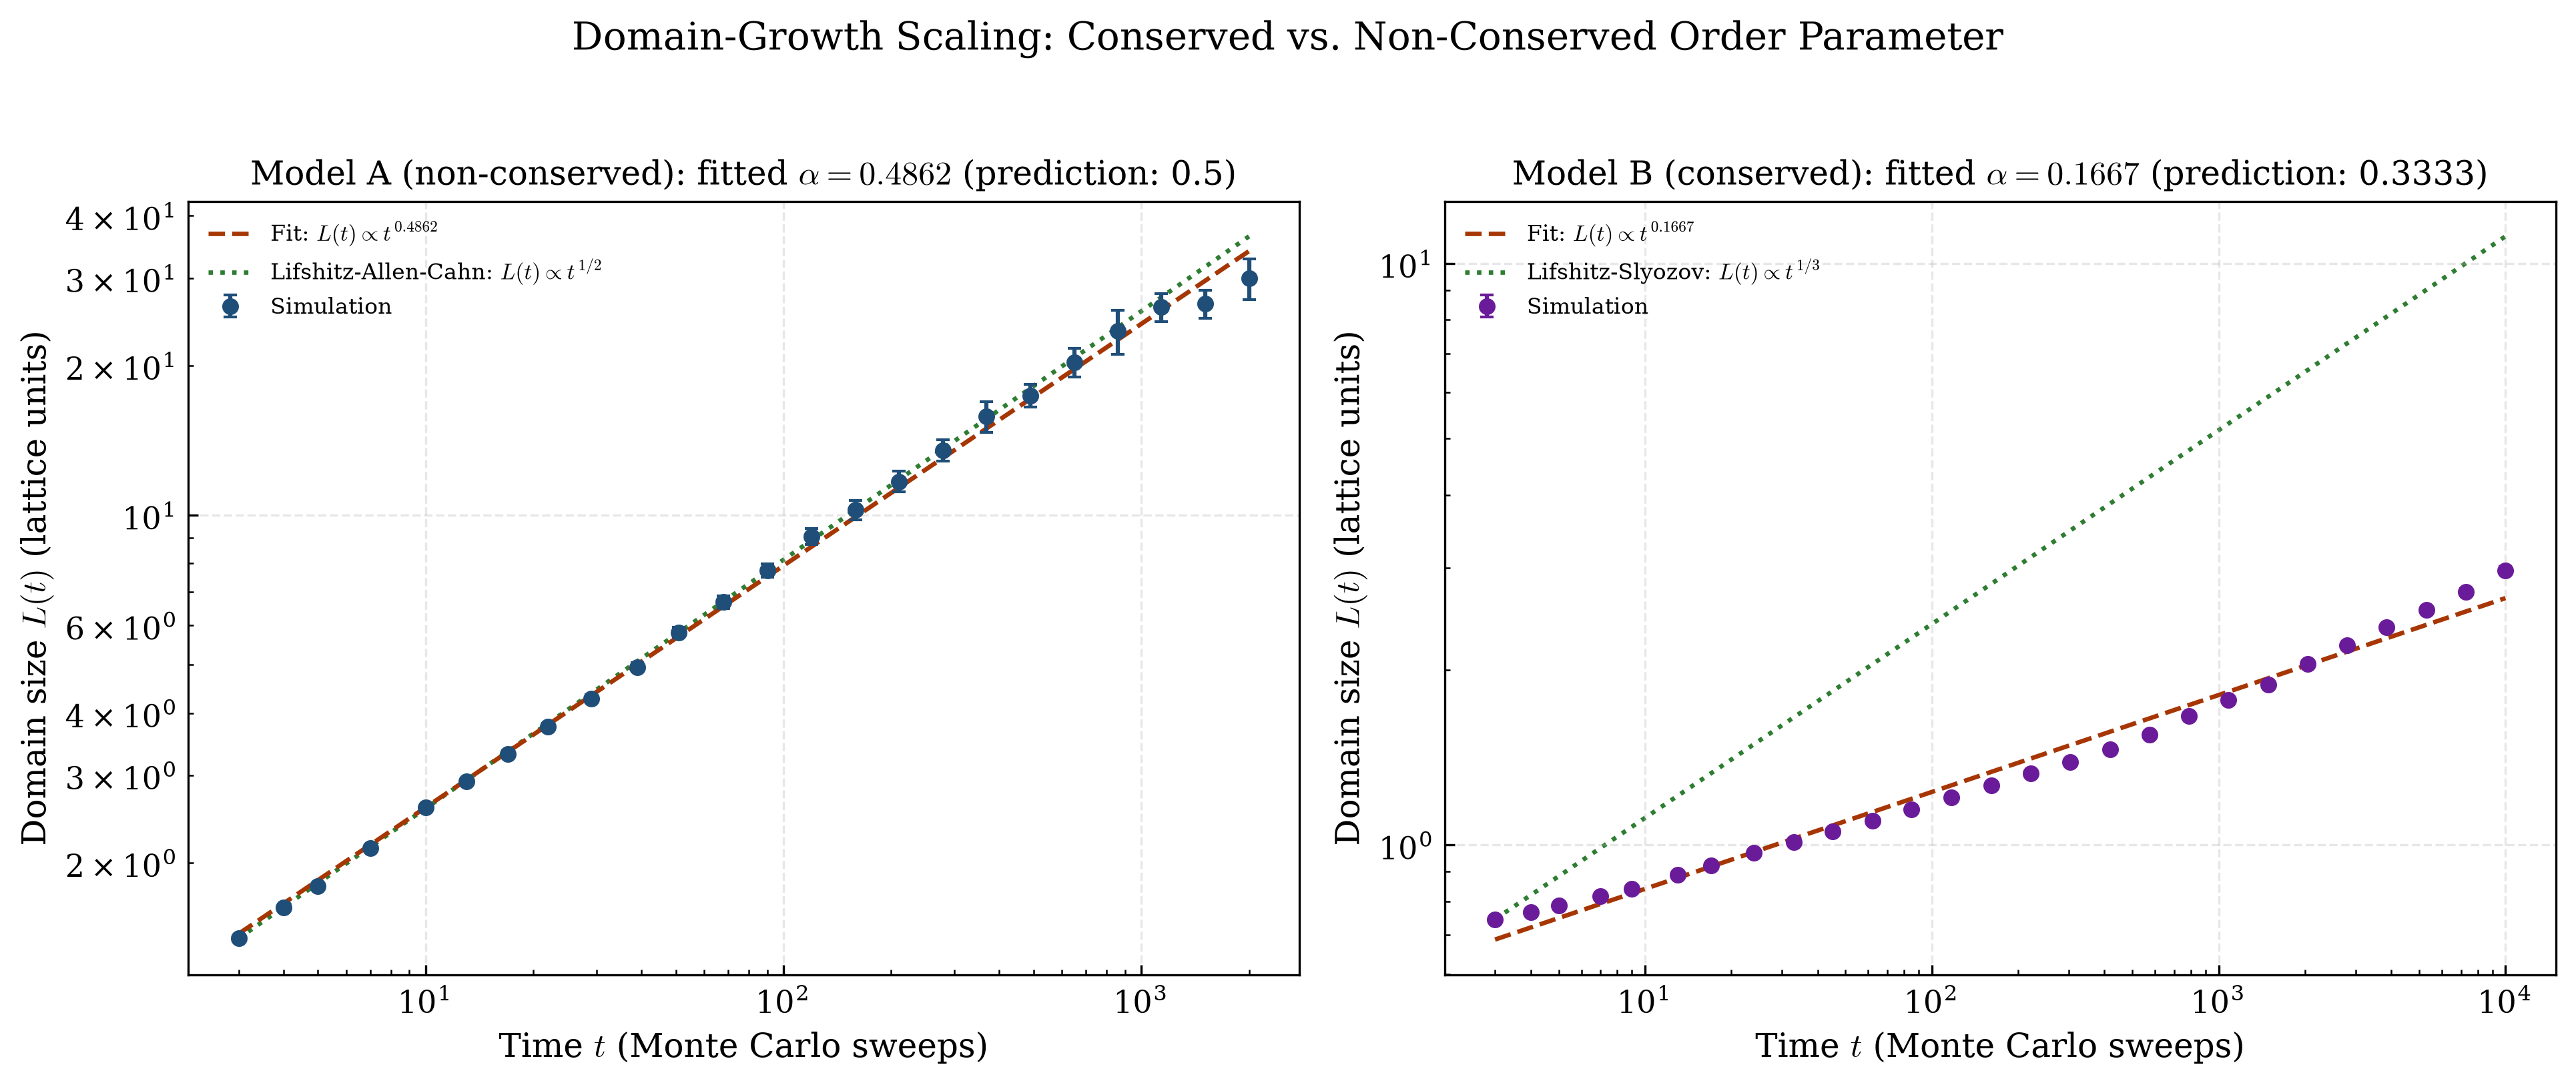
\includegraphics[width=\textwidth]{../figures/fig_comparative_scaling.png}
\caption{Domain size $L(t)$ vs. time on matching log-log axes for Model A
(left) and Model B (right, $L_x$ and $L_y$ averaged), each against its
own theoretical growth law. The visibly shallower Model B slope is a
descriptive comparison under different sizes, couplings and quench
conditions, not a controlled estimate of conservation's causal effect.}
\label{fig:comparative}
\end{figure}

\begin{figure}[t]
\centering
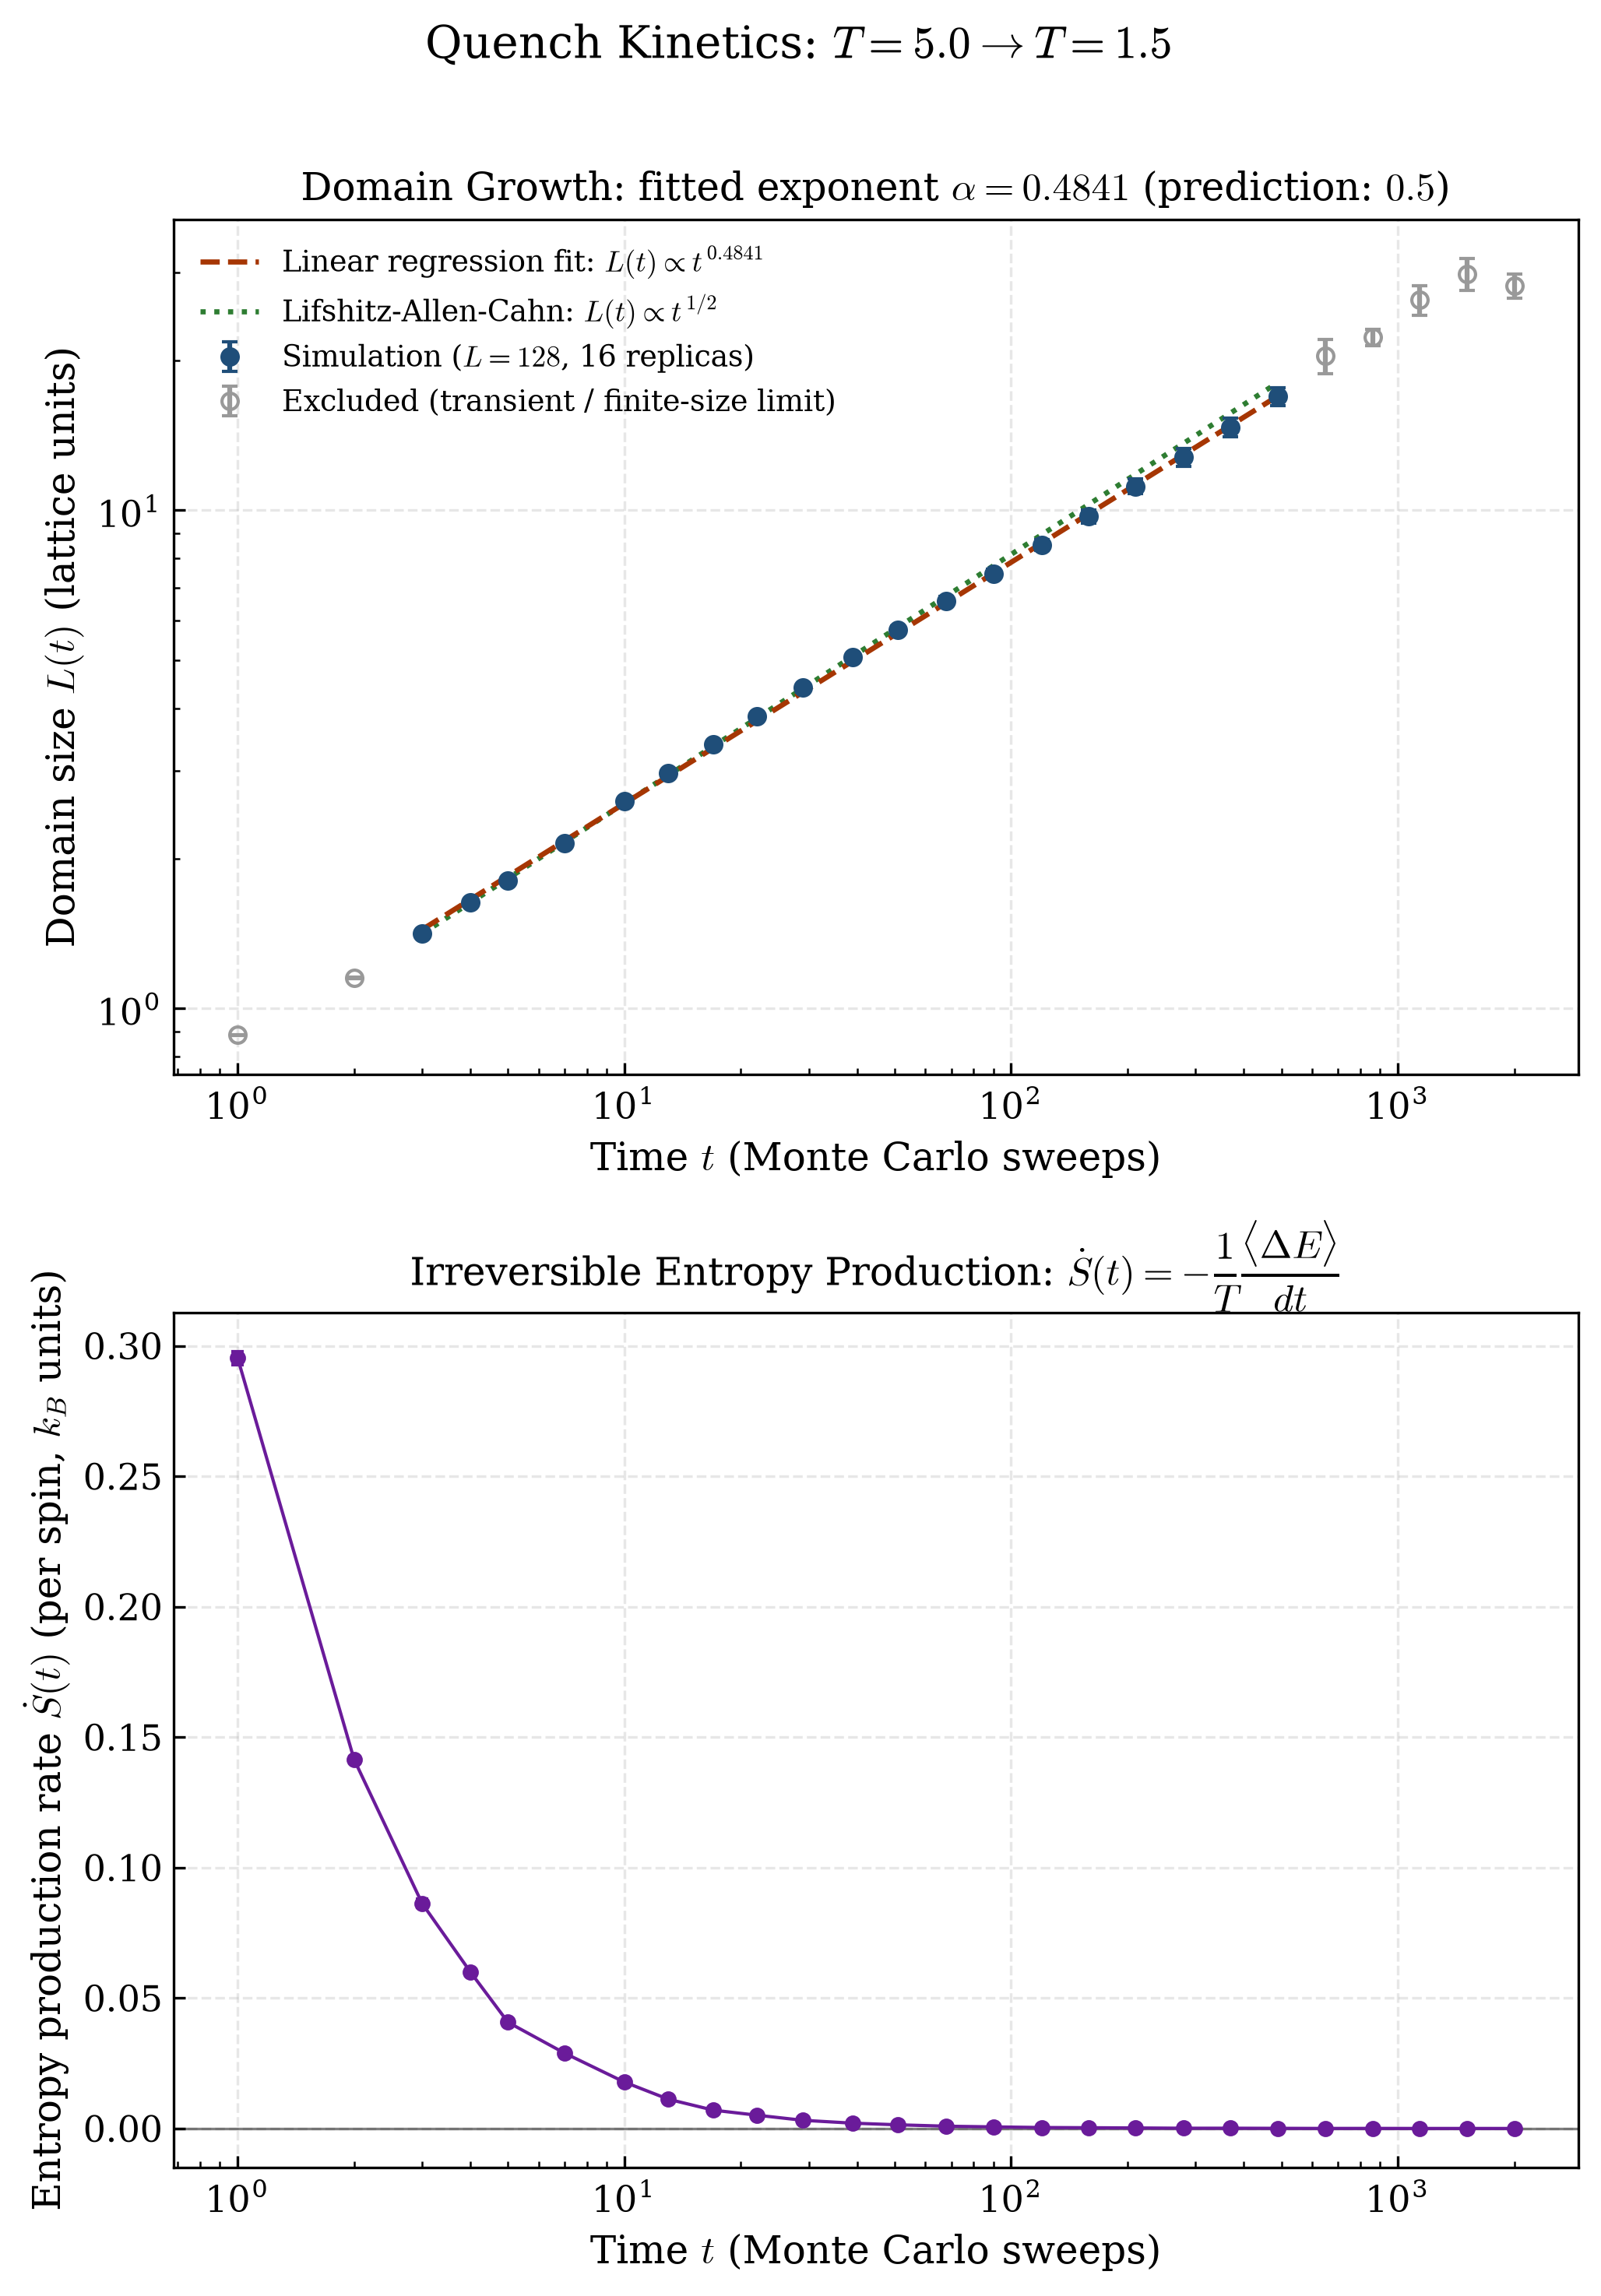
\includegraphics[width=0.85\textwidth]{../model_a/figures/fig3_kinetics_entropy.png}
\caption{Model A quench kinetics ($T_i=5.0\to T_f=1.5$, $L=128$, 16
replicas). \emph{Top:} $L(t)$ with the fitted exponent $\alpha=0.4999$
against the Lifshitz--Allen--Cahn line. \emph{Bottom:} bath entropy-flow
rate $\dot S_{\mathrm{bath}}(t)$ (Section 5), decaying over four orders of
magnitude.}
\label{fig:modela}
\end{figure}

\begin{figure}[t]
\centering
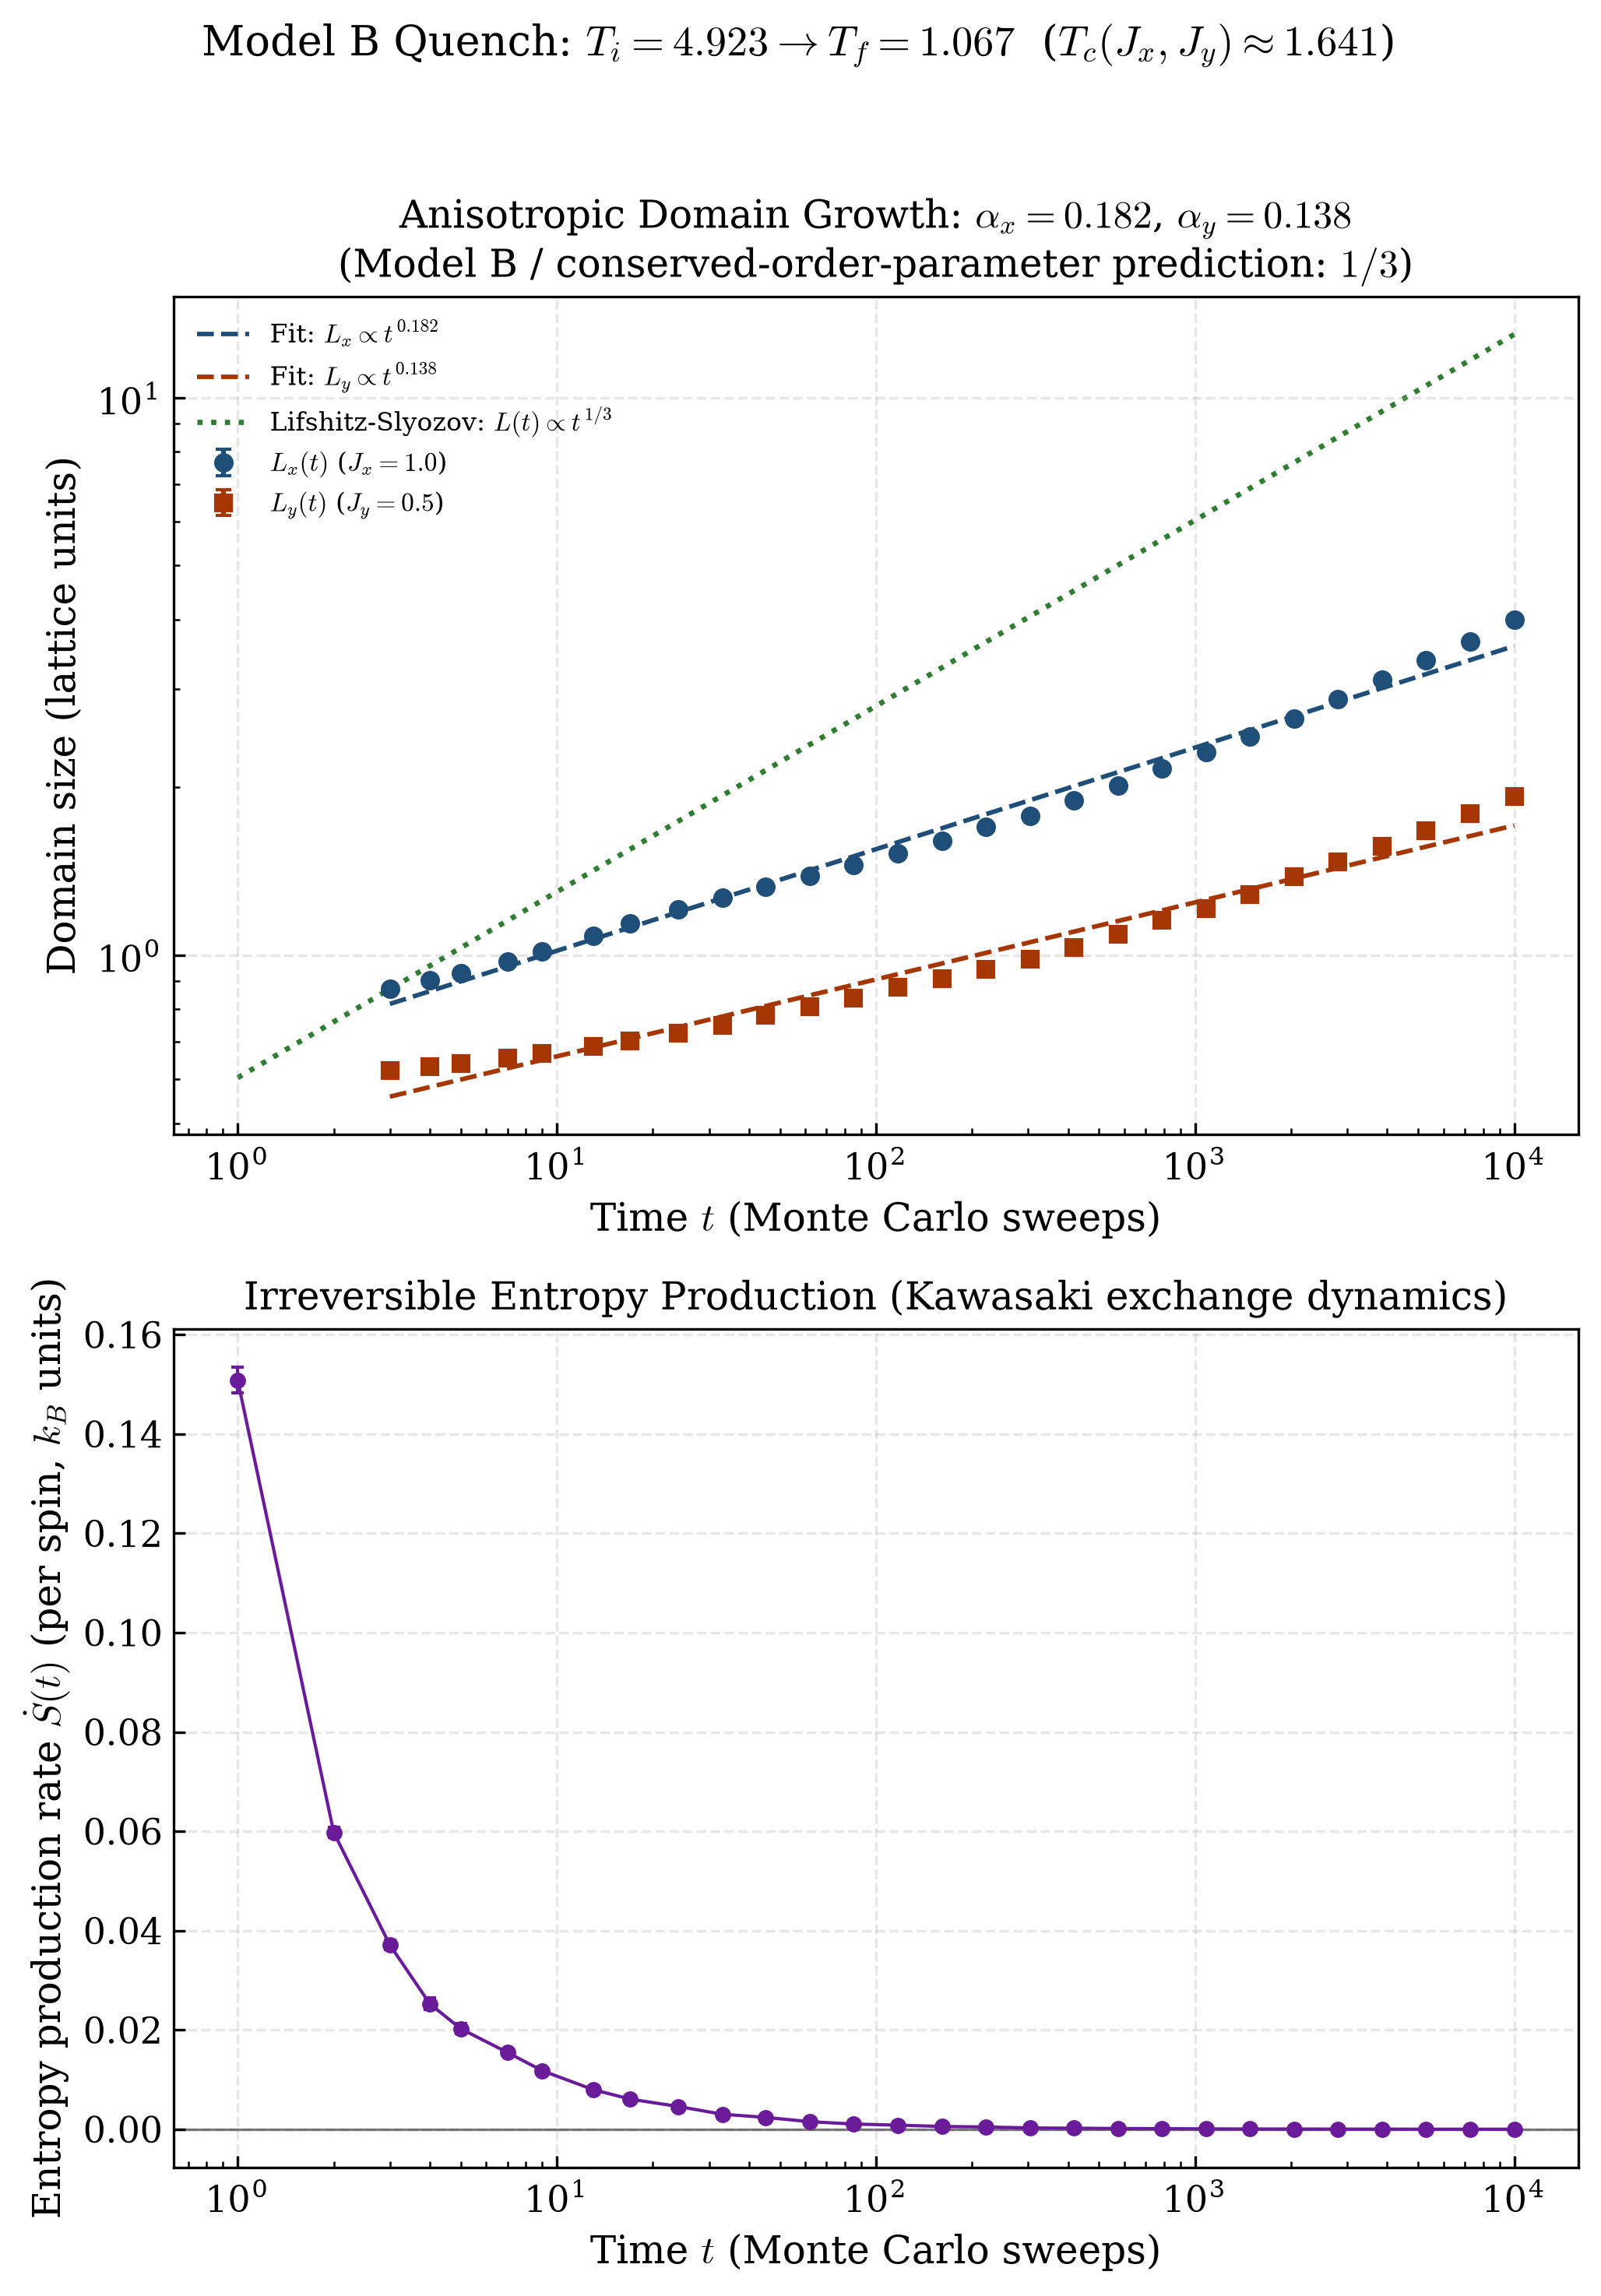
\includegraphics[width=0.85\textwidth]{../model_b/figures/fig_anisotropic_kinetics.png}
\caption{Model B anisotropic quench kinetics ($J_x=1.0$, $J_y=0.5$,
$L=96$, 16 replicas). \emph{Top:} $L_x(t)$ growing visibly faster than
$L_y(t)$, reflecting the stronger horizontal coupling. \emph{Bottom:}
bath entropy-flow rate, again decaying over several orders of magnitude.}
\label{fig:modelb}
\end{figure}

\section{Diagnostic Techniques and Anisotropy}

The autocorrelation function used above, Eq.~\eqref{eq:autocorr}, is a
real-space picture of the microstructure. Its Fourier partner, the
\textbf{structure factor}
\begin{equation}
S(\mathbf{k},t) = \left|\mathcal{F}\{\sigma(\mathbf{r},t)\}\right|^2,
\label{eq:structurefactor}
\end{equation}
is exactly the power spectrum already computed as an intermediate step in
Eq.~\eqref{eq:wiener-khinchin}, and is the natural $k$-space picture of
the same microstructure -- for an isotropic, statistically self-similar
domain pattern, $S(\mathbf{k},t)$ forms a ring at $|\mathbf{k}|\sim
1/L(t)$, shrinking towards the origin as domains coarsen. Under
anisotropic coupling this ring is expected to distort into an ellipse,
elongated along the axis with the \emph{weaker} coupling (since a smaller
$|\mathbf{k}|$ there corresponds to a larger real-space domain size along
that direction). I have not built a dedicated visualisation of this ring
into the software -- doing so is a natural next step -- but the
equivalent, and physically identical, information is already captured
directly in the anisotropic domain sizes $L_x(t) \neq L_y(t)$ plotted in
Fig.~\ref{fig:modelb}, which is the real-space cross-section through
exactly that ellipse along its two principal axes.

The physical picture here is directional coarsening: the horizontal domains
grow roughly twice as fast as the vertical ones by the end of the run
($L_x\approx4.1$ vs.\ $L_y\approx1.9$ lattice units at $t=10{,}000$
sweeps). Real materials can also develop directional microstructures, but
rolling and stress-driven $\gamma'$ rafting involve mechanisms absent from
this fixed-bond lattice. The comparison is about shape and the question
anisotropy raises, not predictive equivalence.

\section{Concentration Dependence: Testing the Limits of Universality}
\label{sec:concentration}

Every result so far has used a symmetric, $50/50$ quench: equal numbers of
$+1$ and $-1$ spins to start, so the minority and majority phases are the
same size. Real phase separation is rarely this symmetric -- an alloy
might be $95\%$ solvent and $5\%$ solute, and the two limits look
completely different under a microscope. Near $50/50$, both phases stay
interconnected and coarsen as a single bicontinuous, sponge-like network
(\emph{spinodal decomposition}); far from $50/50$, the minority phase
breaks up into isolated droplets that coarsen by shrinking and vanishing
individually while the survivors grow. This is a late-stage morphology,
not by itself proof of how the droplets first formed. It would be reasonable to
expect a morphology change this dramatic to come with a different growth
exponent -- and, before checking the literature carefully, I expected
exactly that. It is not what the theory actually predicts, and checking
it properly against both the theory and this project's own simulations
turned out to be more instructive than either of the two more obvious
answers.

\subsection{The prediction: exponent set by conservation, not composition}

A. J. Bray's review of phase-ordering kinetics states the result for
conserved dynamics plainly: ``for off-critical quenches of conserved
systems, the growth law is independent of the volume fraction of the
phases, but the scaling functions are not'' \cite{Bray1994}. The argument
behind this (attributed there to Huse) is a direct extension of the
chemical-potential argument already used for Eq.~\eqref{eq:lifshitz-slyozov}:
the diffusive current that grows a domain of size $L$ scales as
$1/L^2$ regardless of whether that domain is a wall of a bicontinuous
network or the surface of an isolated droplet, so the resulting growth
law $L(t)\propto t^{1/3}$ never referenced the minority-phase volume
fraction in the first place. What \emph{does} depend on volume fraction is
the \emph{scaling function} -- the detailed shape of the correlation
function or the droplet-size distribution -- and, in the strict dilute
limit, the classic three-dimensional Lifshitz--Slyozov--Wagner (LSW)
theory gives a closed-form droplet-size reference under its assumptions
\cite{LifshitzSlyozov1961}. This is worth being
precise about, because it is also the point at which a popular but
imprecise version of this story goes wrong: it is tempting to read
``bicontinuous network'' and ``isolated droplets'' as two different
\emph{growth laws}, when the theory says they are two different
\emph{morphologies of the same growth law}. This section tests that
claim within a finite window, in the actual lattice model simulated throughout this
report rather than in the continuum limit Bray's argument is stated in.

\subsection{A methodological subtlety: choosing a correlation observable for each model}

Extracting $L(t)$ off-critical exposed a real bug in the correlation-based
method used everywhere above. Equation~\eqref{eq:autocorr} assumes the two
phases are equally represented; away from $50/50$ the raw correlation
function no longer decays to zero at large separation but instead
plateaus at $m^2$, where $m$ is the mean magnetization -- and once
$m^2 > 0.5$ (roughly $c \lesssim 0.15$ or $c \gtrsim 0.85$), it never
crosses the $0.5$ threshold Eq.~\eqref{eq:autocorr}'s extraction method
looks for, and every domain-size measurement silently returns \texttt{NaN}.
The standard fix is the \emph{connected} correlation function,
\begin{equation}
g(r,t) = \frac{\langle \sigma_i(t)\,\sigma_{i+r}(t)\rangle - m(t)^2}{1 - m(t)^2},
\label{eq:connected-corr}
\end{equation}
which isolates the fluctuation/domain-structure part of the correlation
and is renormalised so $g(0,t)=1$, matching the convention the raw
correlation already used at $m=0$.

The instructive part is that this is the chosen fix for Model B, not a
definition to impose automatically on Model A. Applying it uniformly to
both models first (my initial approach) changed
the already-verified Model A baseline in Section~3.3, dropping the fitted
exponent from $0.4999$ to $0.379$ -- a large enough shift that comparing
against that section's own previously-established number caught it
immediately. The reason is a genuine physical distinction, not a coding
slip: in Model B, Kawasaki exchange conserves $m$ \emph{exactly}, so
$m(t)=m(0)=2c-1$ for the entire run and subtracting it removes a
constant composition background. In Model A, magnetisation is not conserved;
its magnitude can change as finite replicas order below $T_c$. Subtracting
$m(t)^2$ is mathematically possible, but it defines a different observable
and changed the previously reported Model A baseline. Eq.~\eqref{eq:connected-corr}
is therefore used for the Model B off-critical length below; Model A keeps
the raw correlation, Eq.~\eqref{eq:autocorr},
unchanged, and its off-critical quenches are better understood as a
transient initial bias that ordinary (non-conserved) coarsening dynamics
washes out rather than as a genuine steady off-critical state.

\subsection{Growth exponent vs.\ concentration}

With Eq.~\eqref{eq:connected-corr} in place, I re-ran the quench-kinetics
pipeline at six initial concentrations, $c \in \{0.50, 0.35, 0.25, 0.15,
0.10, 0.06\}$, for both models ($c=0.15$ marks Bray's approximate
threshold below which the minority phase is a disconnected droplet
population rather than a network \cite{Bray1994}; $c=0.06$ sits well
inside it). Model B ran isotropically ($J_x=J_y=1$, $L=96$, 12 replicas,
8000 sweeps) so the concentration effect is not entangled with the
anisotropy study in Section~4; Model A used the same $128\times128$,
$T_i=5.0\to T_f=1.5$ setup as Section~3.3, at 10 replicas and 2500 sweeps.
Figure~\ref{fig:concentration} shows the result.

\begin{figure}[t]
\centering
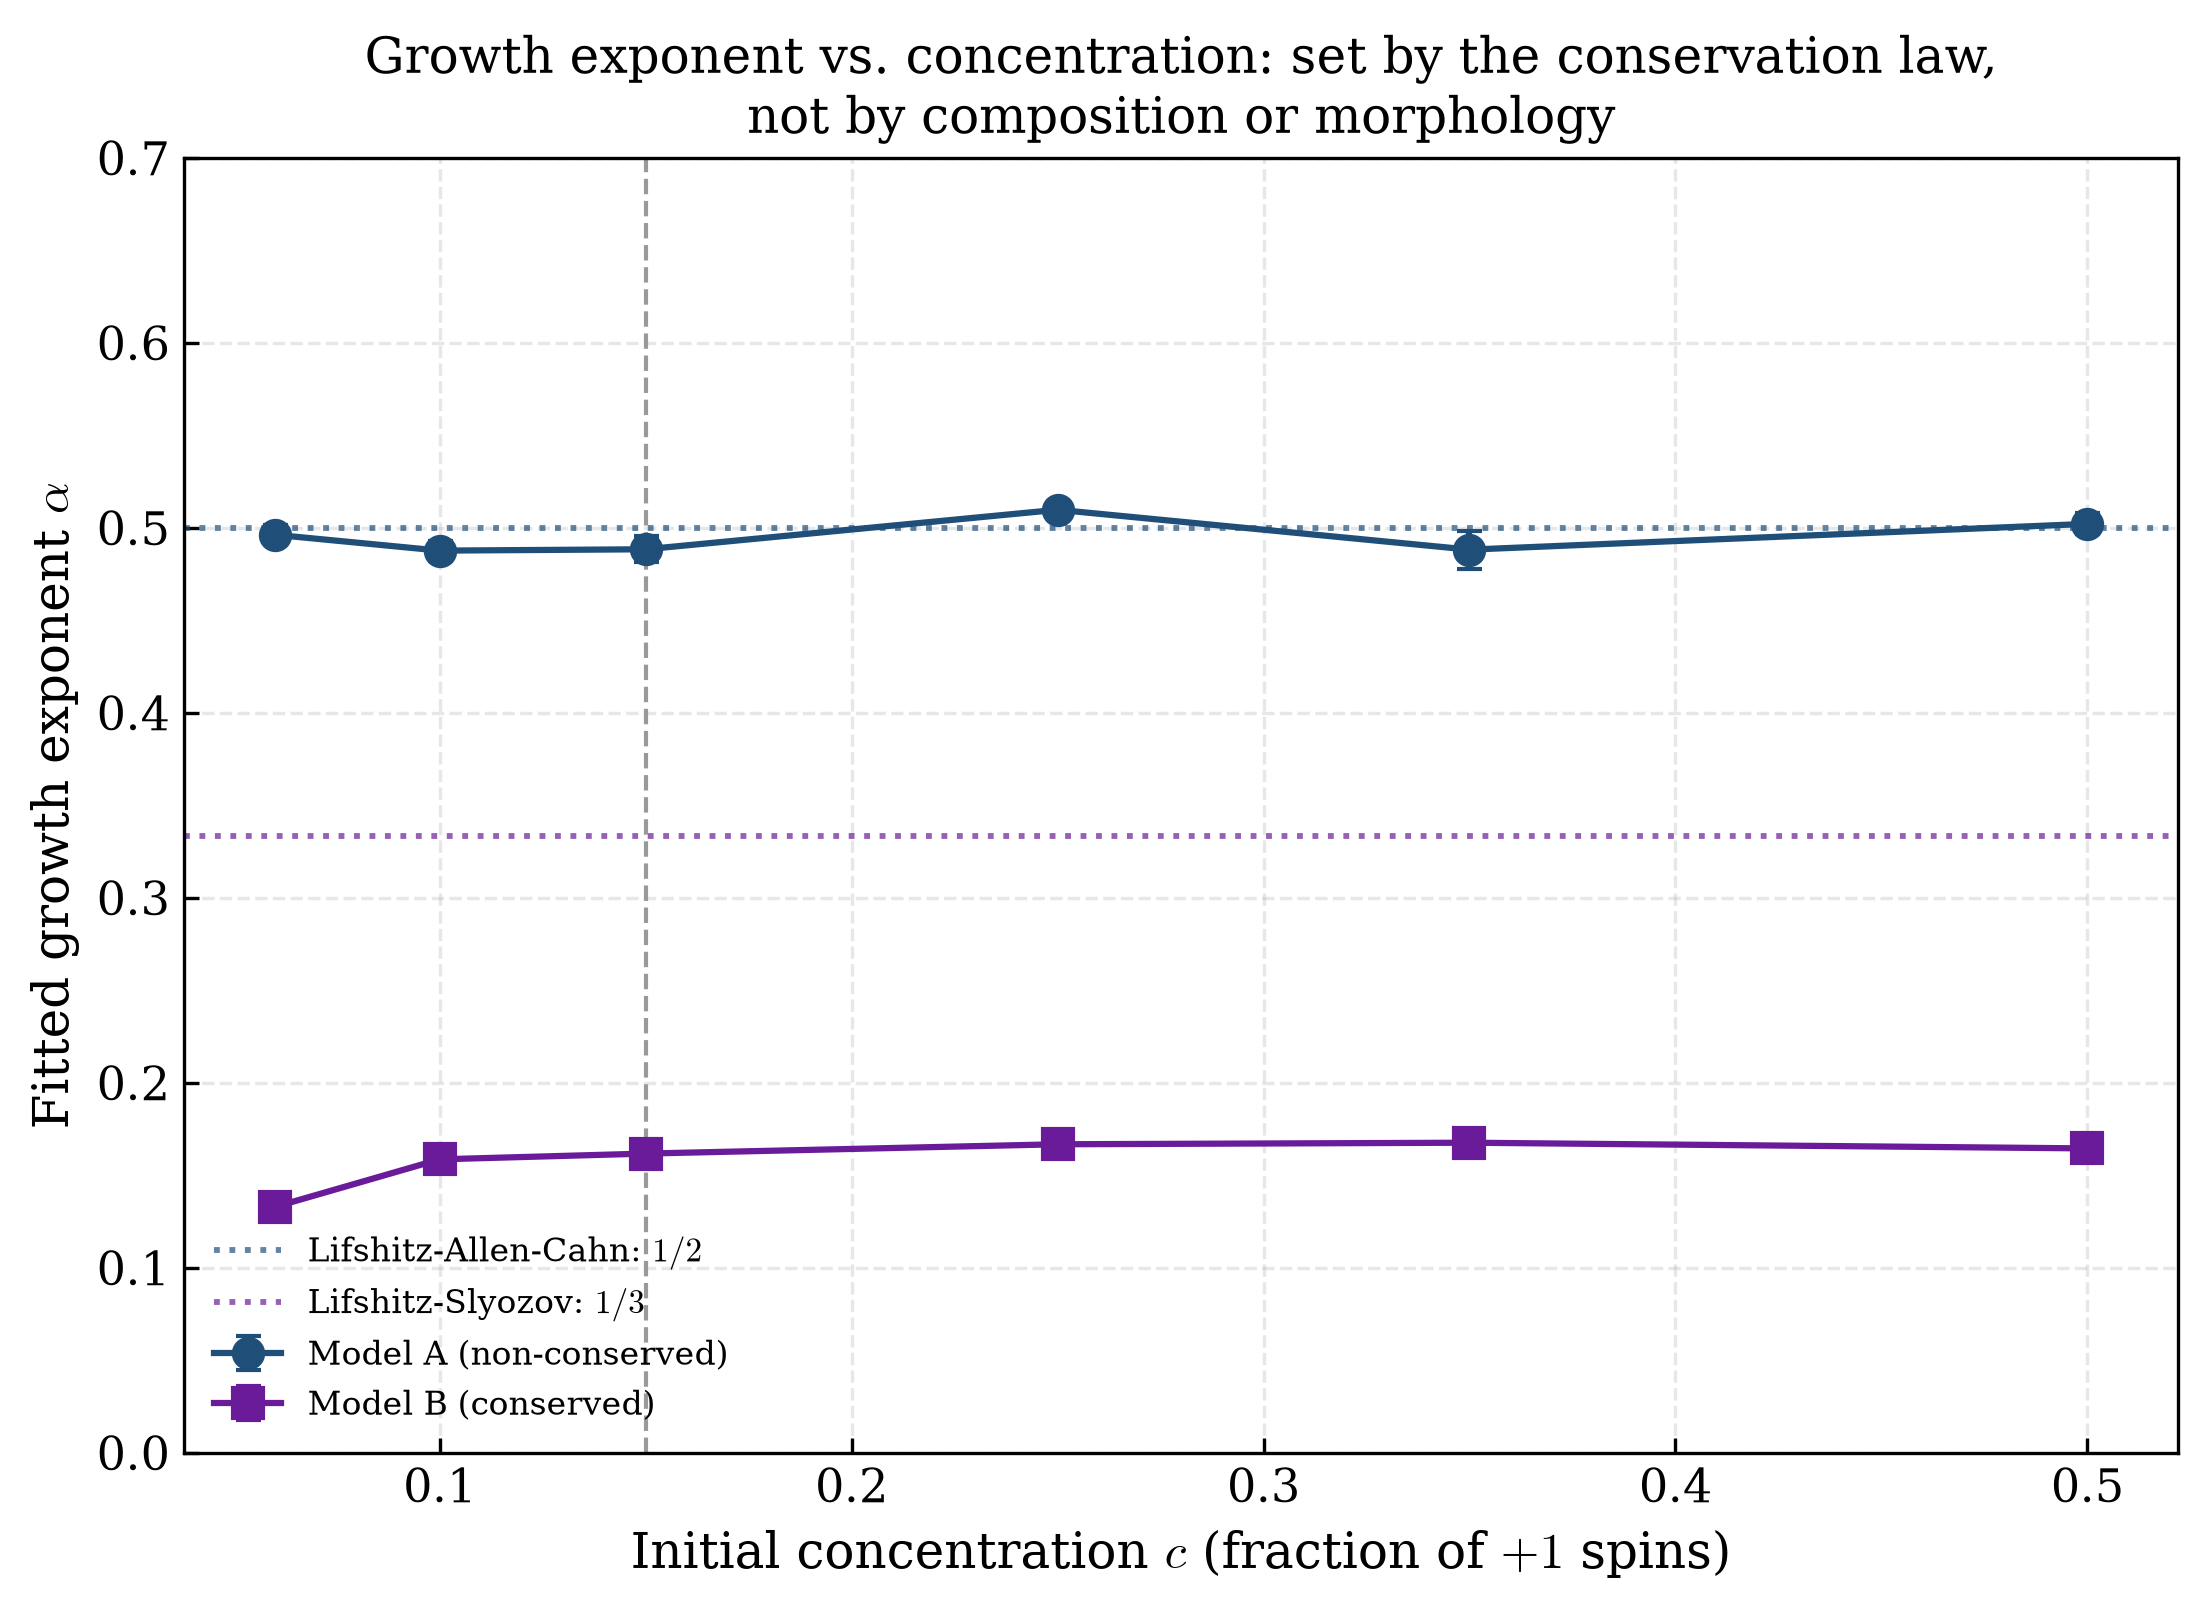
\includegraphics[width=0.85\textwidth]{../figures/fig_concentration_universality.png}
\caption{Fitted growth exponent vs.\ initial concentration for both
models. Model A (non-conserved) sits on $\alpha\approx0.5$ at every
concentration tested, from $0.488$ to $0.510$. Model B (conserved) sits
on a lower, finite-window plateau ($\alpha\approx0.16$--$0.17$ for
$c\ge0.10$) that is flat across the bicontinuous-to-droplet transition,
with a further mild slowing at the most dilute point tested ($c=0.06$,
$\alpha\approx0.133$). Neither model shows the large, discrete jump in
exponent that a ``different growth law for droplets'' hypothesis would
predict.}
\label{fig:concentration}
\end{figure}

For Model A the fitted exponent averages $\alpha = 0.495$, with a
spread of $\pm0.009$ (standard deviation) across all six concentrations
(individual values $0.502$, $0.488$, $0.510$, $0.488$, $0.488$, $0.496$
from $c=0.50$ down to $c=0.06$) -- indistinguishable from $1/2$ at every
concentration tested, well within run-to-run Monte Carlo noise. This is the expected control result given Section 3.1's
argument: curvature-driven wall motion does not care which phase is in
the minority, so as long as \emph{some} interface is present to move,
Model A coarsens at the same rate regardless of composition. For Model B
the fitted exponent is markedly lower than the asymptotic $1/3$
prediction at every concentration -- consistent with the same
pre-asymptotic shortfall already documented for the anisotropic baseline
in Section~3.3 -- but, critically, it stays on essentially the same
plateau ($0.1645$, $0.1676$, $0.1667$, $0.1617$, $0.1586$) across five of the
six concentrations spanning the entire bicontinuous-to-droplet
transition, before dropping further to $0.133$ at the most dilute point.
That residual drop is itself informative rather than a contradiction: it
is consistent with the well-documented fact that conserved coarsening's
corrections to its asymptotic growth law are unusually strong and
long-lived \cite{Bray1994}, and there is every reason to expect those
corrections to be strongest exactly where the fewest, most widely
separated droplets have to communicate across the largest distances --
i.e., in the most dilute regime, at fixed lattice size and run length.
Within the simulated time and size window, the data do not show a clear
jump to a different stable exponent plateau. These finite-window measurements
are compatible with a shared asymptotic growth law, but do not establish it.
A finite-size and longer-time study is required to distinguish
composition-dependent transients, estimator effects and saturation from
an asymptotic change in exponent.

\subsection{A qualitative benchmark against Fe--Cr ageing data}

Fe--Cr provides a useful experimental point of contact because its
low-temperature miscibility gap produces Fe-rich $\alpha$ and Cr-rich
$\alpha'$ regions and is associated with the industrially important
``475\,$^\circ$C embrittlement'' phenomenon. Xu \emph{et al.} combined
small-angle neutron scattering (SANS), atom-probe tomography, and electron
microscopy for Fe--Cr alloys aged at 773\,K and reported an effective growth
exponent of $0.16$ for the inverse SANS peak position (the decomposition
wavelength) in their alloy labelled 35Cr; a Guinier particle-radius analysis gave
$R\propto t^{0.27}$ \cite{Xu2016}. The present $c=0.35$ conserved-model run
gives $\alpha=0.1676\pm0.0008$ as a fit standard error, not uncertainty
from independent replicas or a choice of fitting window
(Figure~\ref{fig:fecr-benchmark}). The experimental composition table uses
weight percent, not the model's site fraction: these compositions are not
matched, and proximity of the exponents is not evidence of agreement.

\begin{figure}[t]
\centering
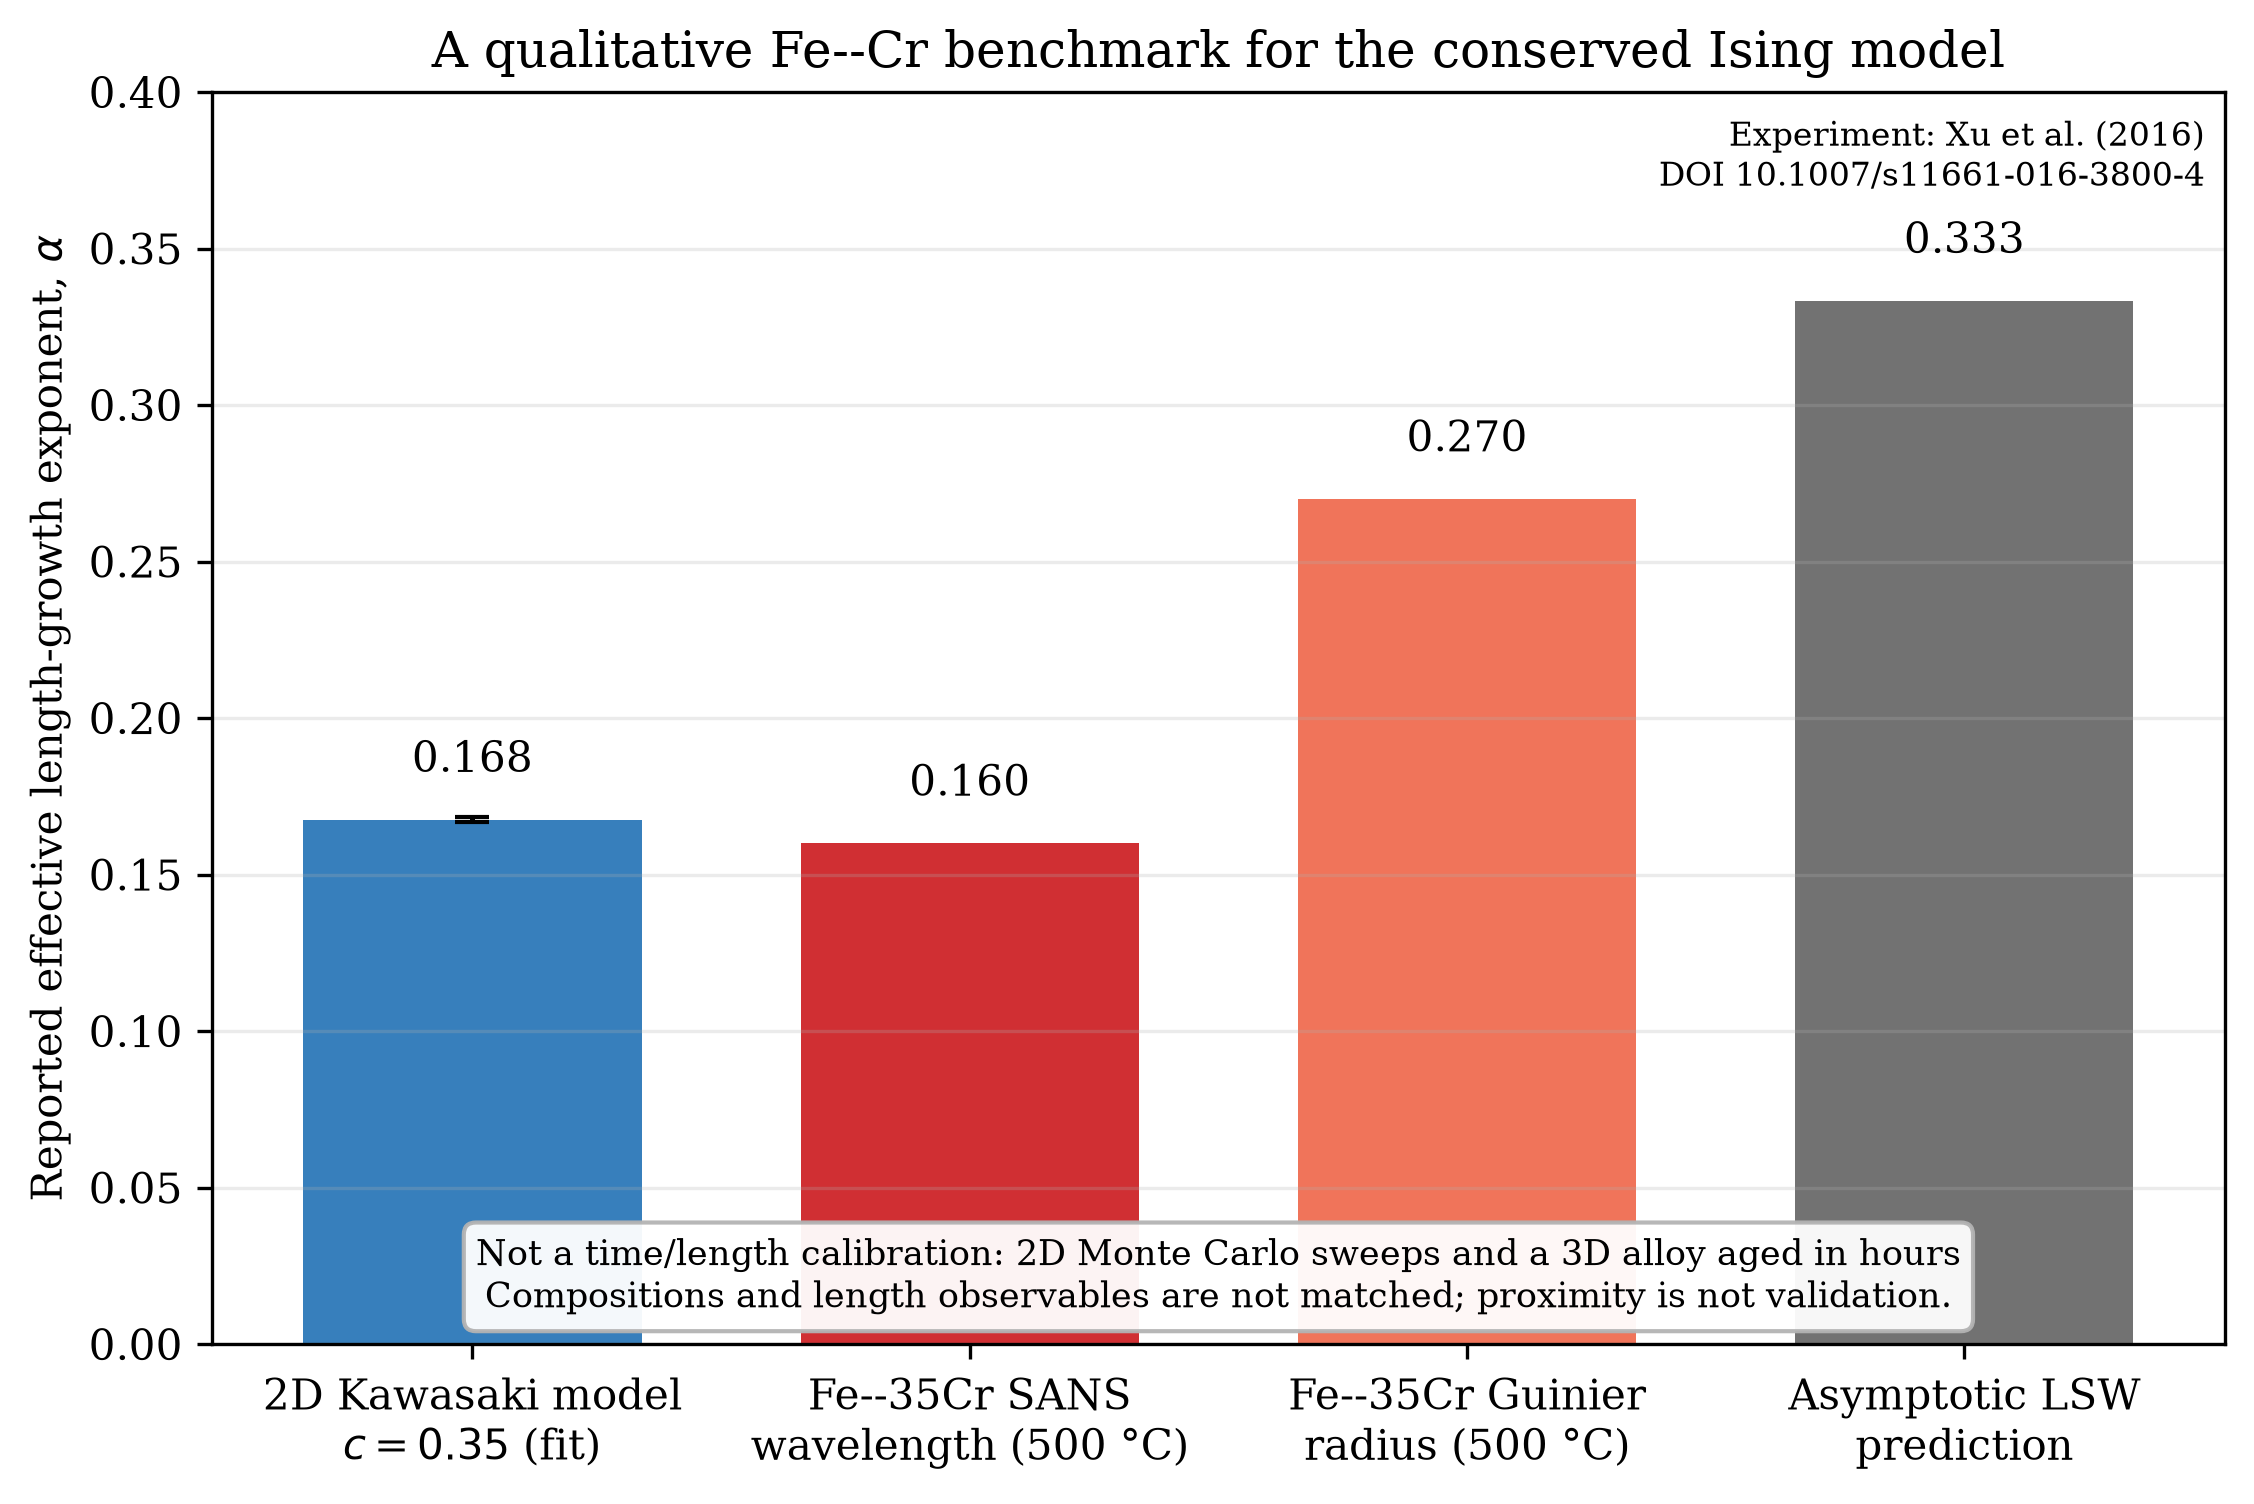
\includegraphics[width=0.9\textwidth]{../figures/fig_fecr_literature_benchmark.png}
\caption{Qualitative comparison of the Model B $c=0.35$ effective exponent,
two published Fe--35Cr measures at 773\,K, and the asymptotic LSW value. The
similarity of the first two values motivates a shared pre-asymptotic question;
it is not a dimensional calibration or quantitative validation.}
\label{fig:fecr-benchmark}
\end{figure}

This numerical proximity must not be over-interpreted. The simulation is a
two-dimensional, nearest-neighbour lattice with Monte Carlo sweeps as
algorithmic time; the experiment is a three-dimensional alloy aged in hours,
and the two experimental observables themselves give different effective
exponents. The defensible connection is therefore the question rather than a
parameter fit: both systems show regime-dependent effective exponents below
$1/3$, making finite-time diagnostics and careful choice of length-scale
estimator important. A quantitative Fe--Cr model would require, at minimum,
three-dimensional geometry, calibrated free energy and mobility, and a mapping
to physical length and time.

\subsection{Droplet-size distribution vs.\ Lifshitz--Slyozov--Wagner theory}

The complementary half of Bray's statement -- that the \emph{scaling
function}, not the growth law, is where concentration leaves its mark --
is directly testable in the dilute regime, where LSW theory gives an
exact closed form for the droplet-size distribution. Writing $u=R/\langle
R\rangle$ for a droplet's radius scaled by the mean radius at a given
time,
\begin{equation}
g(u) = \frac{3^4 e}{2^{5/3}}\, u^2\, \frac{\exp\!\left[-1/(1-2u/3)\right]}{(u+3)^{7/3}(3/2-u)^{11/3}}, \qquad 0 \le u < \tfrac{3}{2},
\label{eq:lsw-distribution}
\end{equation}
and $g(u)=0$ for $u\ge3/2$ \cite{LifshitzSlyozov1961} -- a genuinely
distinctive shape, since the hard cutoff at $u=3/2$ (no droplet may exceed
$1.5$ times the mean size) has no analogue in a generic unimodal
distribution like a Gaussian or log-normal. I extracted the simulated
droplet-size distribution at $c=0.06$ by labelling connected minority-spin
clusters (implemented with periodic boundary stitching, since a plain
connected-component labeller would spuriously split or duplicate droplets
that straddle the lattice edge), pooling $513$ droplets of at least $4$
sites across 30 independent replicas at the final sampled sweep, and
converting each cluster's area to an effective radius via $R=\sqrt{\text{area}/\pi}$.
Figure~\ref{fig:lsw} compares the result to Eq.~\eqref{eq:lsw-distribution}.

\begin{figure}[t]
\centering
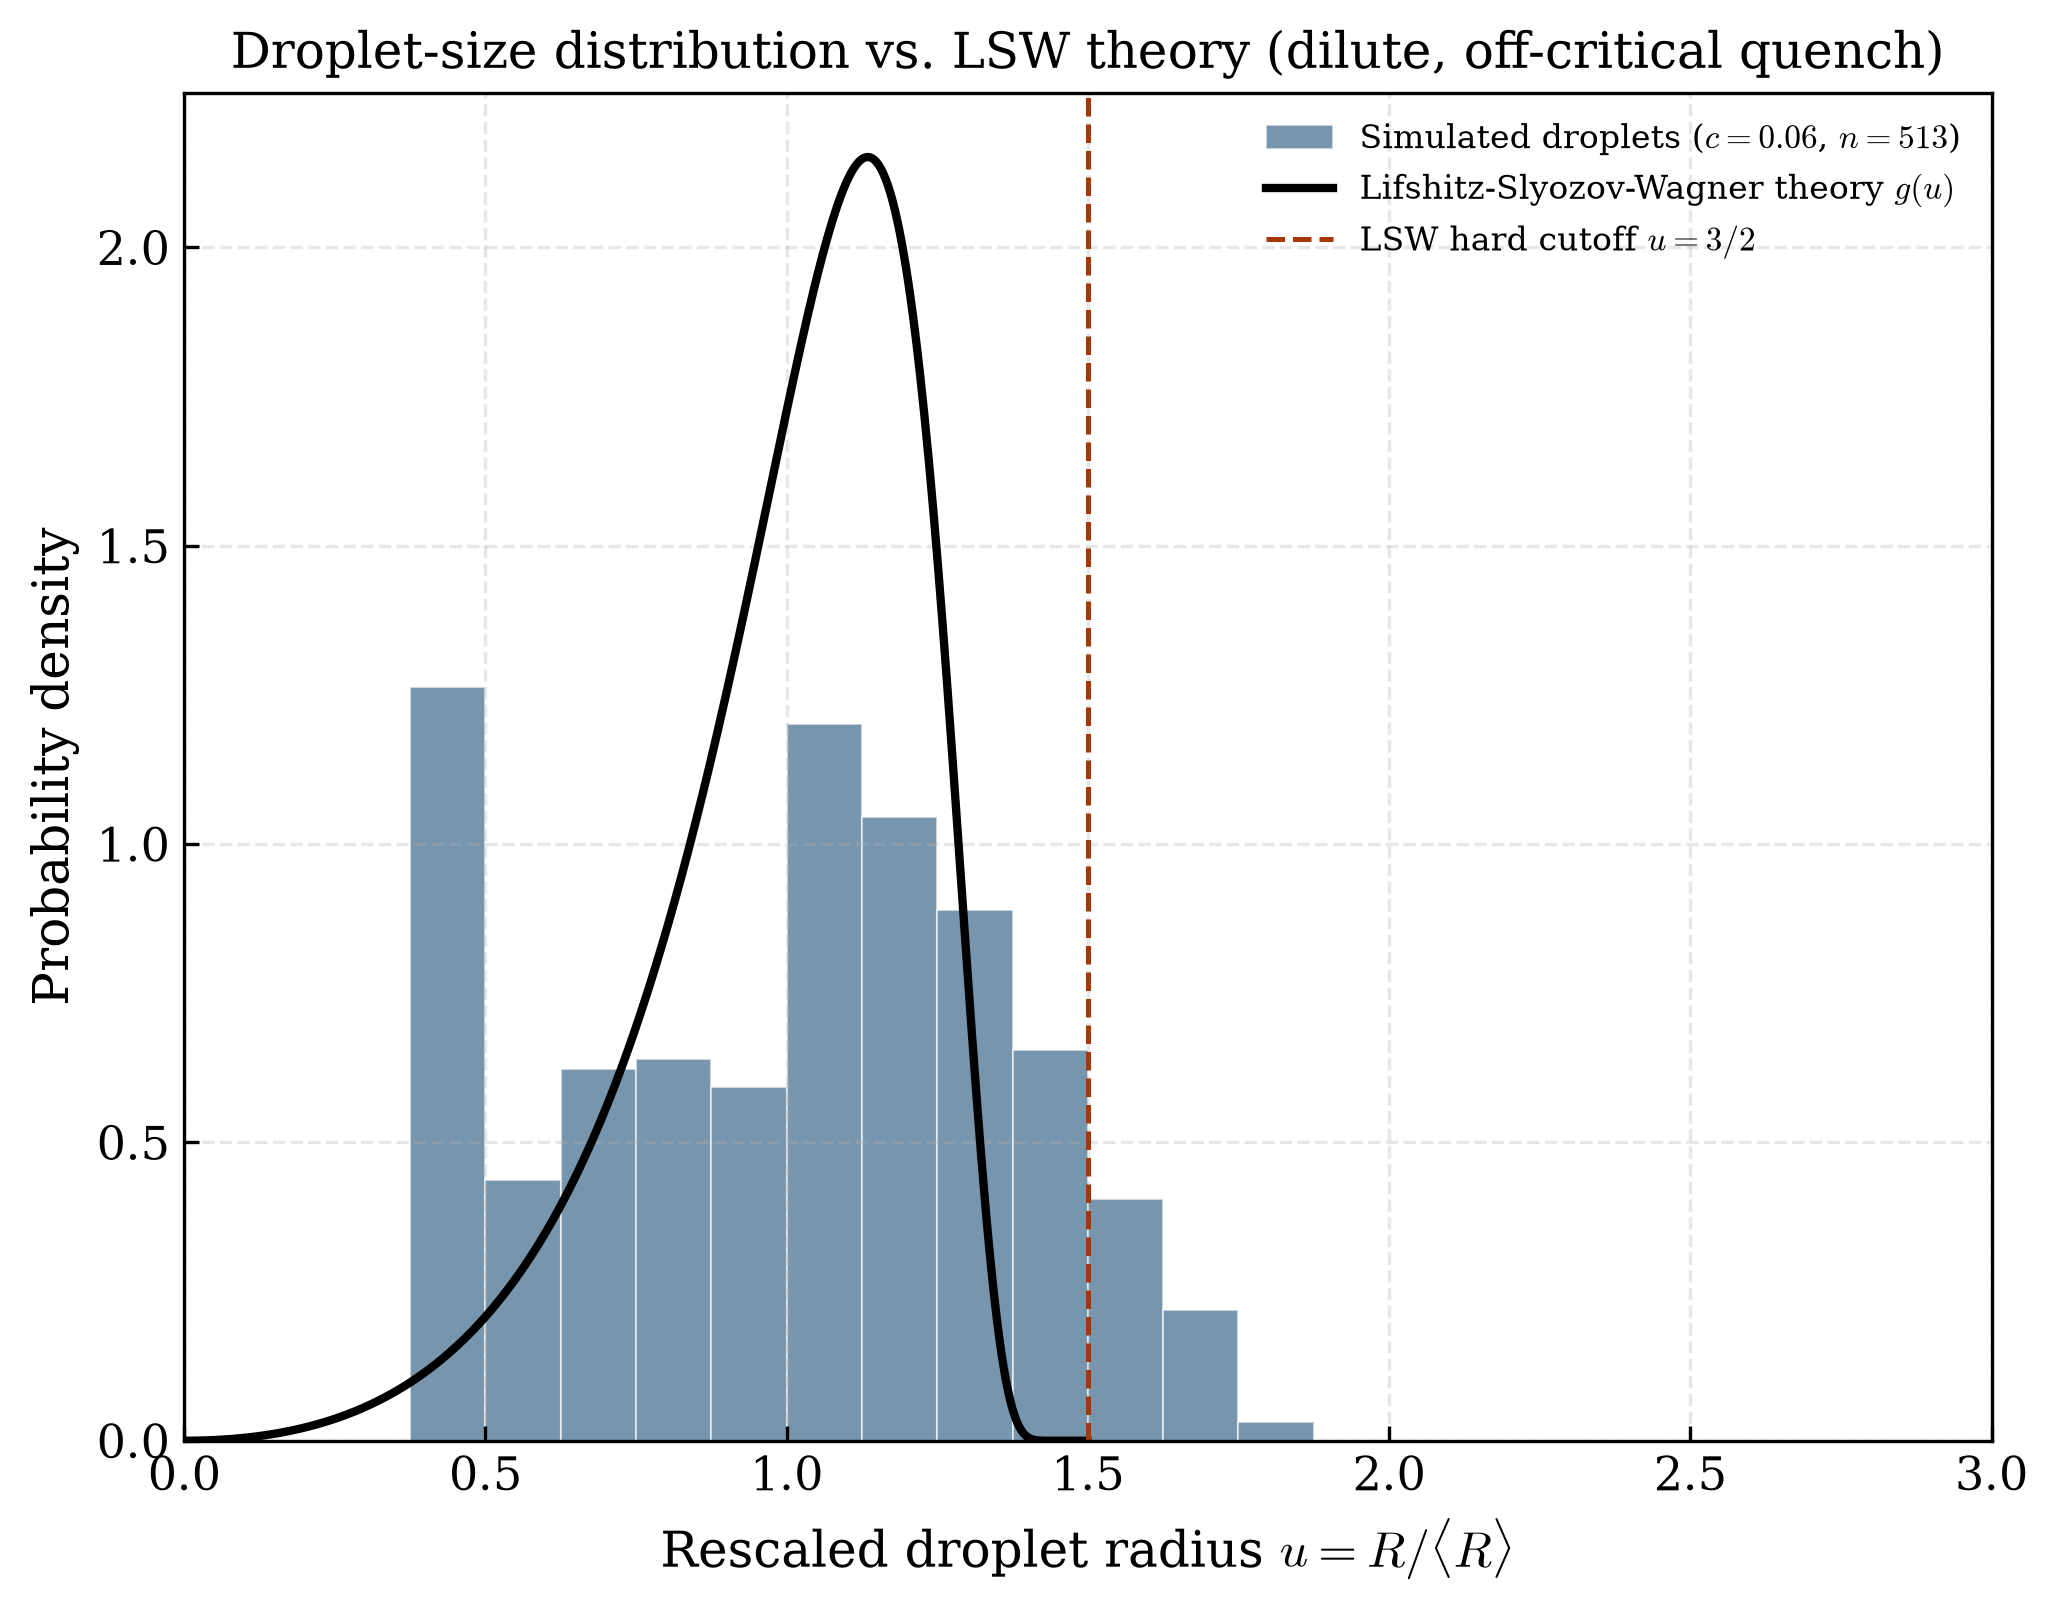
\includegraphics[width=0.7\textwidth]{../model_b/figures/fig_droplet_size_distribution_lsw.png}
\caption{Simulated droplet-radius distribution at $c=0.06$ ($n=513$
droplets, 30 pooled replicas) against the closed-form LSW prediction,
Eq.~\eqref{eq:lsw-distribution}. The simulated distribution reproduces
the qualitative signature of LSW theory -- a single asymmetric peak near
$u\approx1$--$1.3$ rather than a symmetric or long-tailed shape -- but
visibly departs from the exact dilute-limit prediction in two ways: an
excess of small droplets below $u\approx0.5$, and a tail of droplets
beyond the strict LSW cutoff $u=3/2$.}
\label{fig:lsw}
\end{figure}

The reference distribution is not an exact prediction for this finite,
two-dimensional lattice. The classical LSW expression describes dilute
three-dimensional droplets in an asymptotic regime, whereas the measured
objects here are finite connected clusters with a lattice-dependent radius
definition. Finite concentration, incomplete scaling, coalescence and the
cluster estimator could all contribute to the discrepancies. A size
histogram alone cannot distinguish them. In particular, assigning the
large-droplet tail to coalescence would require tracking actual merger
events, and assigning small clusters to newly formed droplets would require
time-resolved evidence. The comparison is therefore qualitative; it is not
a verification of the LSW distribution in two dimensions.

\subsection{Synthesis}

The two move rules give different measured coarsening rates, while changing
composition changes morphology and has a smaller effect on the measured
exponents over much of the tested range. These observations motivate a
test of Bray's asymptotic prediction; they do not yet confirm composition
independence of the asymptotic exponent. Nucleation and spinodal decomposition
also have distinct early-stage mechanisms. A possible shared late-stage
growth exponent does not make those mechanisms equivalent.

\section{Bath Entropy Flow and Interfacial Dissipation}

Because the Metropolis rule couples the lattice to an implicit heat bath
held at fixed temperature $T_f$, every accepted move that changes the
system's energy by $\Delta E$ delivers heat $Q = -\Delta E$ to that bath,
by simple conservation of energy. Summing the accepted $\Delta E$ within
each time interval $dt$ (in sweeps) and averaging over replicas gives the
per-spin bath entropy-flow rate (in the code's $k_B=1$ units),
\begin{equation}
\dot S_{\mathrm{bath}}(t) = -\frac{1}{N T_f}\,\frac{\langle \Delta E\rangle}{dt},
\label{eq:entropy}
\end{equation}
where $N=L^2$ and $\Delta E$ is the total lattice-energy change over the
checkpoint interval. The historical output field is named
\texttt{entropy\_production} but stores this bath-flow proxy. Computing it
requires no simulation beyond the bookkeeping the Metropolis step is
already doing. It is not, by itself, the total stochastic entropy
production $\dot S_{\mathrm{tot}}=\dot S_{\mathrm{sys}}+\dot
S_{\mathrm{bath}}$: estimating the system's ensemble Shannon-entropy change
would require an additional calculation. For Model A,
$\dot S_{\mathrm{bath}}(t{=}1)\approx0.297$ immediately
after the quench, falling to $\approx9.8\times10^{-6}$ by $t=2000$ sweeps
-- over four orders of magnitude. For Model B,
$\dot S_{\mathrm{bath}}(t{=}1)\approx0.149$
falls to $\approx6.5\times10^{-6}$ by $t=10{,}000$ sweeps -- again over
four orders of magnitude. In both cases the interpretation is the same:
immediately after the quench the lattice is riddled with domain walls and
misaligned spins, so a large fraction of proposed moves are strongly
energetically favourable and get accepted; as coarsening proceeds and
interfacial area shrinks, fewer moves are favourable, and dissipation
falls in step with it. The transition rule used to produce this result
obeys detailed balance at fixed temperature (Section~2.3); the observed
positive, decaying
$\dot S_{\mathrm{bath}}(t)$ is a property of the replica-averaged,
coarse-grained relaxation trajectory, not of every single move
-- a concrete illustration of how macroscopic irreversibility emerges
from reversible microscopic rules once one considers the statistically
overwhelming direction of an ensemble's evolution, the standard
resolution to Boltzmann's $H$-theorem \cite{Huang1987} restated here in
the language of stochastic thermodynamics \cite{Seifert2012}.

\section{Implications for Materials Design, and Conclusion}

The materials connection is useful because an alloy's properties depend
partly on the size, spacing and shape of its phases. Conserving the
composition makes the spin-exchange model a better starting point for
thinking about binary phase separation than single-spin flips. It does
not supply a processing recipe or a lifetime prediction. The familiar
$t^{1/3}$ coarsening argument concerns a late-stage, diffusion-limited
regime under specific assumptions; the lower slopes measured here are
finite-window results, not evidence that a real alloy will age more
slowly. Cahn--Hilliard phase-field models also use a conserved order
parameter \cite{CahnHilliard1958}, but they can include thermodynamics and
transport missing from this nearest-neighbour lattice. The useful
comparison is the shared conservation constraint and the need to define
the measured length carefully, not quantitative equivalence.

To summarise: I built two Monte Carlo engines in the Ising framework,
one with a non-conserving elementary move and one with a conserving one.
The historical baseline runs also differ in size, coupling and quench,
so their slopes do not isolate the effect of that move rule.
The non-conserved model coarsens close to the predicted $t^{1/2}$ rate;
the conserved model coarsens more slowly, with an effective exponent below
the diffusion-limited $t^{1/3}$ prediction. The present runs have not
quantitatively accounted for that discrepancy. Making the conserved model's
coupling anisotropic produces directionally elongated domains through unequal
bond costs; it does not model elastic rafting or measured crystallographic
texture. The concentration sweep gives an approximately flat *effective*
exponent down to $c=0.10$, followed by additional slowing at $c=0.06$.
That finite-window pattern does not establish composition independence of
the asymptotic exponent. The dilute droplet-size distribution has some
qualitative resemblance to the closed-form Lifshitz--Slyozov--Wagner
reference, but differs in shape and support; the reference is not an exact
prediction for this finite, two-dimensional lattice. Tracking
the heat exchanged with the thermal bath at every accepted move gives a
consistently defined measurement of bath entropy flow in both cases, falling
by several orders of magnitude as each system relaxes. Computing total
stochastic entropy production remains a distinct extension because it also
requires the system-entropy term.
The source code, selected completed simulation archives, analysis outputs,
and both interactive dashboard implementations are openly available
\cite{CodeRepo}. The dashboards have not been deployed as research instruments.

\begin{thebibliography}{99}

\bibitem{Onsager1944} L. Onsager, Crystal Statistics. I. A Two-Dimensional Model with an Order-Disorder Transition, Phys. Rev. \textbf{65}, 117 (1944).

\bibitem{Metropolis1953} N. Metropolis, A. W. Rosenbluth, M. N. Rosenbluth, A. H. Teller, and E. Teller, Equation of State Calculations by Fast Computing Machines, J. Chem. Phys. \textbf{21}, 1087 (1953).

\bibitem{HohenbergHalperin1977} P. C. Hohenberg and B. I. Halperin, Theory of Dynamic Critical Phenomena, Rev. Mod. Phys. \textbf{49}, 435 (1977).

\bibitem{Lifshitz1962} I. M. Lifshitz, Kinetics of Ordering During Second-Order Phase Transitions, Sov. Phys. JETP \textbf{15}, 939 (1962).

\bibitem{AllenCahn1979} S. M. Allen and J. W. Cahn, A Microscopic Theory for Antiphase Boundary Motion and Its Application to Antiphase Domain Coarsening, Acta Metall. \textbf{27}, 1085 (1979).

\bibitem{LifshitzSlyozov1961} I. M. Lifshitz and V. V. Slyozov, The Kinetics of Precipitation from Supersaturated Solid Solutions, J. Phys. Chem. Solids \textbf{19}, 35 (1961).

\bibitem{Kawasaki1966} K. Kawasaki, Diffusion Constants near the Critical Point for Time-Dependent Ising Models, Phys. Rev. \textbf{145}, 224 (1966).

\bibitem{CahnHilliard1958} J. W. Cahn and J. E. Hilliard, Free Energy of a Nonuniform System. I. Interfacial Free Energy, J. Chem. Phys. \textbf{28}, 258 (1958).

\bibitem{Bray1994} A. J. Bray, Theory of Phase-Ordering Kinetics, Adv. Phys. \textbf{43}, 357 (1994).

\bibitem{Seifert2012} U. Seifert, Stochastic Thermodynamics, Fluctuation Theorems and Molecular Machines, Rep. Prog. Phys. \textbf{75}, 126001 (2012).

\bibitem{Huang1987} K. Huang, \textit{Statistical Mechanics}, 2nd ed. (Wiley, New York, 1987).

\bibitem{Xu2016} X. Xu \emph{et al.}, Structural Characterization of Phase Separation in Fe--Cr: A Current Comparison of Experimental Methods, Metall. Mater. Trans. A \textbf{47}, 5942 (2016), doi:10.1007/s11661-016-3800-4.

\bibitem{CodeRepo} Code and data available at \url{https://github.com/djangothompson12-alt/ising-monte-carlo}.

\end{thebibliography}

\end{document}
